%! Author = Quentin
%! Date = 12/01/2020

\documentclass[
10pt, % The default document font size, options: 10pt, 11pt, 12pt
%oneside, % Two side (alternating margins) for binding by default, uncomment to switch to one side
english, % ngerman for German
singlespacing, % Single line spacing, alternatives: onehalfspacing or doublespacing
%draft, % Uncomment to enable draft mode (no pictures, no links, overfull hboxes indicated)
%nolistspacing, % If the document is onehalfspacing or doublespacing, uncomment this to set spacing in lists to single
%liststotoc, % Uncomment to add the list of figures/tables/etc to the table of contents
%toctotoc, % Uncomment to add the main table of contents to the table of contents
%parskip, % Uncomment to add space between paragraphs
%nohyperref, % Uncomment to not load the hyperref package
headsepline, % Uncomment to get a line under the header
%chapterinoneline, % Uncomment to place the chapter title next to the number on one line
%consistentlayout, % Uncomment to change the layout of the declaration, abstract and acknowledgements pages to match the default layout
]{MastersDoctoralThesis} % The class file specifying the document structure

\usepackage[utf8]{inputenc} % Required for inputting international characters
\usepackage[T1]{fontenc} % Output font encoding for international characters

% \usepackage{mathpazo} % Use the Palatino font by default

% \usepackage[backend=biber,style=authoryear,natbib=true]{biblatex} % Use the bibtex backend with the authoryear citation style (which resembles APA)
% \addbibresource{bibliography.bib} % The filename of the bibliography
% \usepackage{natbib}
% \bibliographystyle{plainnat}
% \bibliography{blabla}
% \usepackage[autostyle=true]{csquotes} % Required to generate language-dependent quotes in the bibliography

%----------------------------------------------------------------------------------------
%	MARGIN SETTINGS
%----------------------------------------------------------------------------------------

\geometry{
    paper=a4paper, % Change to letterpaper for US letter
    inner=1.2cm, % Inner margin
    outer=2.5cm, % Outer margin
    bindingoffset=.5cm, % Binding offset
    top=1.5cm, % Top margin
    bottom=1.5cm, % Bottom margin
%showframe, % Uncomment to show how the type block is set on the page
}

\frontmatter % Use roman page numbering style (i, ii, iii, iv...) for the pre-content pages

\pagestyle{plain} % Default to the plain heading style until the thesis style is called for the body content

\usepackage{epfml}
\newcommand\independent{\protect\mathpalette{\protect\independenT}{\perp}}
\newcommand{\independenT}[2]{\mathrel{\rlap{$#1#2$}\mkern2mu{#1#2}}}
\newcommand{\concatx}{\left[ X, \tilde{X} \right]}

\DeclareMathOperator{\swap}{swap}


\begin{document}

    % \setlength{\parindent}{0pt}
    \setlength{\parskip}{0pt} %(needs to be before titlepage and frontmatter to keep the table of contents lists short)
    \frontmatter
    \newgeometry{centering,margin=1.5cm}

\begin{titlepage}
\begin{center}

% \sffamily
% \fontfamily{stix}\selectfont

\null\vspace{2cm}

\begin{figure}[H]
	\centering
	\begin{subfigure}{.5\textwidth}
		\centering
		
\includegraphics[width=0.6\linewidth]{figures/epfl.pdf}
	\end{subfigure}%
	\begin{subfigure}{.5\textwidth}
		\centering
		
\includegraphics[width=0.6\linewidth]{figures/inria_pms.pdf}
	\end{subfigure}
\end{figure}

\vspace{2cm}

\textsc{\Large Master of data science}\\[8pt]
\textsc{\large Machine Learning and Optimization laboratory}\\[2pt]
\textsc{\large Master project}\\

\vspace{1cm}

\rule{0.85\textwidth}{1.5pt}\\[8pt]
{\huge \textbf{High-dimensional knockoff feature selection}}\\[6pt]
{\Large Scalable false discovery rate control}\\[2pt]
\rule{0.85\textwidth}{1.5pt}\\

\vspace{2cm}

School of Computer and Communication Sciences\\
École Polytechnique Fédérale de Lausanne\\
\vspace{1cm}
Master thesis of\\[3pt]
\textbf{Quentin Rebjock}\\
\vspace{1.2cm}
\small
Supervised by the professors%
\begin{align*}
	&\text{Alexandre d'Aspremont (Sierra team, Inria, ENS, CNRS)}\\
	&\text{Martin Jaggi (Machine Learning and Optimization lab, EPFL)}\\[24pt]
\end{align*}
Paris, Inria, March 2020

\end{center}
\end{titlepage}

\restoregeometry

    \setcounter{page}{0}
    \newgeometry{centering,margin=1.5cm}
\thispagestyle{empty}
\markboth{Acknowledgements}{Acknowledgements}
\renewcommand{\abstractname}{Acknowledgements}
\null\vspace{10cm}
\phantomsection
\begin{abstract}
    \addcontentsline{toc}{chapter}{Acknowledgements} % adds an entry to the table of contents
    \centering
    \begin{minipage}[b]{\dimexpr\paperwidth-10cm}
        I would like to thank my master thesis advisor Alexandre d'Aspremont who gave me the opportunity to
        work.
        I would also like to thanks Armin Askari and Laurent El Ghaoui with whom I had the opportunity to work,
        and who provided substantial help for the resolution of SDP problems.
        More generally, to the people I met at Sierra and Willow.
        Finally, I would like to thank my EPFL advisor Martin Jaggi for his support.
    \end{minipage}
\end{abstract}
\restoregeometry

    \cleardoublepage
%\chapter*{Abstract}
\markboth{Abstract}{Abstract}

\null\vspace{4.5cm}
\phantomsection
\begin{abstract}
\addcontentsline{toc}{chapter}{Abstract} % adds an entry to the table of contents
\centering
\begin{minipage}[b]{\dimexpr\paperwidth-10cm}
      High-dimensional feature selection has become a common task in many sciences over the past decades
      because of advancements in data acquisition.
      It is now possible to record dozens of thousands of features at low cost,
      and it is crucial to find out later which of them are of interest.
      In this master thesis, we focus on false discovery rate control,
      that is the problem of making as many relevant selections as possible
      while maintaining the number of false positives under a certain threshold.\\

      Recently~\cite{model_x_knockoffs} introduced the knockoffs framework to control the false discovery rate
      when performing feature selection.
      The key idea is to build a knockoff (fake) feature for each original feature, and compare their significance against
      a statistical model.
      Despite the theoretical possibility to employ this framework in high-dimension, several bottlenecks
      make it unemployable in practice.
      We take advantage of low-rank approximations to efficiently build knockoff features in high dimension,
      and show that a reasonable statistical power can be preserved by using accelerated significance statistics.
      We apply these techniques to genetic data and perform FDR control on roughly
      $35\,000$ features in less than a minute on a standard workstation.\\\\\\

      \textbf{Keywords}: Feature selection, false discovery rate control, knockoff filter, high dimension
\end{minipage}
\end{abstract}

    \cleardoublepage
\chapter*{Notations}
\markboth{Notations}{Notations}
\addcontentsline{toc}{chapter}{Notations}

$\N$ denotes the set of natural integers and $\R$ the set of real numbers.
%
Vectors are written in bold letters, e.g. $\xx, \yy \in \R^p$.
%
Matrices are in capital bold letters, e.g. $\mX \in \R^{n \times p}$.
%
We may cast any vector $\xx \in \R^p$ to a column matrix $x \in \R^{p \times 1}$ with the same entry values.
%
We note $\odot$ the Hadamard (element-wise) product between two vectors or matrices.
%
$\0$ and $\1$ are the vectors whose all entries are $0$ and $1$ respectively, and whose size is inferred by the context.
%
For a vector $\vv$, we note $\norm{\vv}_0$ the number of non-zero entries of $\vv$ (that is, its cardinality).
%
The $\diag$ operator can be used in two contexts;
either to transform a vector into a diagonal matrix whose diagonal entries match the vector,
or to extract the diagonal of a matrix.
For example
\begin{equation*}
    \diag \begin{bmatrix}
         1\\
         2
    \end{bmatrix}
    =
    \begin{bmatrix}
        1 & 0\\
        0 & 2
    \end{bmatrix}
    ,\qquad
    \diag \begin{bmatrix}
        1 & 2\\
        3 & 4
    \end{bmatrix}
    =
    \begin{bmatrix}
         1\\
         4
    \end{bmatrix}
\end{equation*}
%
Given two matrices $A$ and $B$, we note $\big[ A, B \big]$ and $\big[ A; B \big]$ their horizontal and
vertical concatenation respectively (if dimensions match).
%
Functions $\R \to \R$ applied to matrices are implicitly performed element-wise, unless otherwise specified.
%
$\E \cX$ denotes the expectation of a random variable (or vector) $\cX$.

Given a set $\cS$, $\abs{\cS}$ and $\#\cS$ denote its cardinality.


    \cleardoublepage
    \pdfbookmark{\contentsname}{toc}
    \tableofcontents

    % % Following content is OPTIONAL (List of figures + tables)
    % \cleardoublepage
    % \phantomsection
    % \addcontentsline{toc}{chapter}{List of Figures} % adds an entry to the table of contents
    % \listoffigures
    %
    % \cleardoublepage
    % \phantomsection
    % \addcontentsline{toc}{chapter}{List of Tables} % adds an entry to the table of contents
    % \listoftables
    % your list of symbols here, if needed.


    %%%%%%%%%%%%%%%%%%%%%%%%%%%%%%%%%%%%%%%%%%%%%%
    %%%%% MAIN: The chapters of the thesis
    %%%%%%%%%%%%%%%%%%%%%%%%%%%%%%%%%%%%%%%%%%%%%%
    \mainmatter
    \cleardoublepage
\chapter*{Introduction}
\markboth{Introduction}{Introduction}
\addcontentsline{toc}{chapter}{Introduction}

Feature selection is an active area of research in statistics and machine learning
aiming, among others, at making models more interpretable.
The idea is to identify the most relevant observed covariates that best explain a phenomenon.
Often, one is interested in selecting as many pertinent features (true positives) as possible,
that is, maximizing true discoveries,
while maintaining the number of false positives under a certain threshold.
This problem is called false discovery rate control and finds applications in many sciences,
such as biology, economy, medicine and many others.
This is why a multitude of techniques have been developed to this end,
the most widely used being the one proposed by~\cite{bh}.
However, in the past two decades, acquiring massive amounts of data has become increasingly cheaper
and it is now frequent that datasets contain several dozens of thousands of features.
A common practice is to measure as many variables as possible,
and figure out afterwards which of them prove to be valuable.
On top of that, measuring covariates is often simpler than labeling samples with the right categories,
as the latter requires human efforts and can hardly be automatized.
For that reason, many datasets have more features than samples
and it is especially the case in some fields like biology~\citep{statistical_inference_genome},
where genomic and fMRI data contain a huge amount of features but a relatively low number of patients.
In this high dimension setup, feature selection and false discovery rate control are particularly challenging.
The Benjamini–Hochberg procedure requires estimates of independent $p$-values for each feature,
which rapidly becomes hard when the dimension increases,
or may even be impossible.

Recently~\citet{fixed_x_knockoffs} introduced the knockoff framework,
which is a set of procedures capable of performing feature selection,
and that are proven to theoretically control the false discovery rate under mere assumptions.
The key idea is to build a knockoff (that is, fake) feature for each authentic feature,
and compare their significance against a statistical model.
This framework was revisited and extended to a more general inference setting~\citep{model_x_knockoffs},
allowing notably to perform feature selection in the high dimension case,
that is when the number of features is larger than the number of samples.
The generality of this selection procedure
and the fact that many statistical models can be plugged in make it particularly appealing.
However, the construction of the knockoff features and the computation of test statistics
are two costly steps requiring to solve optimization problems whose size grow with the number of features.
Because of these two bottlenecks,
the knockoff framework can hardly be employed in high dimension in practice despite the theoretical guarantees.

In this work, we focus on the high-dimensional knockoff setting and propose techniques
to alleviate the bottlenecks mentioned above.
Constructing quality knockoffs relies on solving a SDP problem
which quickly becomes intractable as the dimension increases.
We propose a coordinate ascent approach with low-rank approximations
that both theoretically and experimentally scale well with the number of features.
Regarding test statistics, recent feature selection models~\citep{sparse_naive_bayes, sparse_center_classifiers}
empirically get close to the performances of the Lasso~\citep{lasso} at very cheap computational cost.
We implement efficiently these algorithms in a publicly available Python package.
In the end, we are able to apply the knockoff framework
in a linear time complexity with respect to the number of dimensions.

This master thesis is organized as follows.
Chapter~\ref{ch:fs} introduces the concepts of feature selection and
false discovery rate control, along with a few techniques that are usually employed.
Chapter~\ref{ch:knockoffs} details the knockoff selection procedure developed by Barber-Candès
and its principal theoretical guarantees.
In Chapter~\ref{ch:sdp},
we focus on the knockoff features constitution part
and propose a log-barrier coordinate ascent algorithm to solve the main bottleneck of the construction.
We show that low-rank covariance approximations considerably speed up the calculations.
Chapter~\ref{ch:fsc} addresses the problem of statistics computation,
and presents a sparse version of naive Bayes, among other things.
Finally, in Chapter~\ref{ch:exp} we detail experiments performed on genetic data and prove the scalability
and efficiency of our methods.

    \cleardoublepage
    \chapter{Feature selection}\label{ch:fs}

We introduce in this chapter the concepts of feature selection and false discovery rate control,
as well as a short review of a few methods that are usually employed,
including the Lasso and Benjamini–Hochberg-Yekutieli procedures.

\section{Background on feature selection}\label{sec:bfs}

\subsection{Definitions}\label{subsec:fs_defs}

Feature selection is an active area of research in statistics and machine learning.
It primarily consists in identifying the most relevant features (or covariates) explaining an observed variable.
It is closely related to Occam's razor which is a principle stating that
the simplest explanation is often the best one.
More formally, let $\cX$ be a $p$-dimensional random vector representing observed features
and $\cY$ a random target that may depend on $\cX$.
For example, $\cX$ could be the levels of expression of the genes of an individual,
and $\cY \in \zoset$ a binary response indicating whether or not the person has some disease.
We wish to find the subset of covariates $\cS \subseteq \fset$ that best explains the target $\cY$,
be it a regression or a classification problem.
To do so, suppose that the joint vector $\left( \cX,\, \cY \right)$ follows some distribution,
that is $\left( \cX,\, \cY \right) \sim \mathcal{P}_{\cX,\, \cY}$.
Even though finding the conditional distribution $\cP_{\cY \mid \cX}$ is beyond hope,
one may be interested in finding on which subset $\cS$ of features $\cP_{\cY \mid \cX}$ depends.
Such a subset is not necessarily unique
\begin{figure}[h]
    \centering
    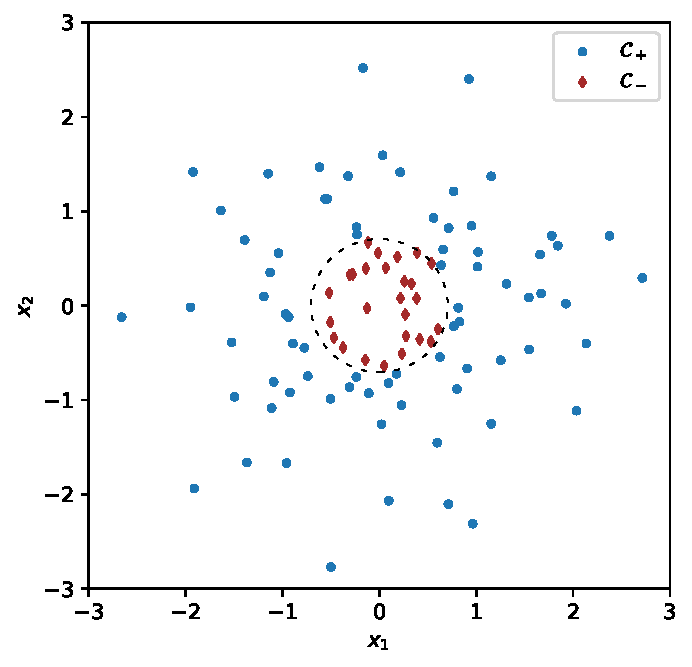
\includegraphics[width=0.4\linewidth]{figures/fs_subset_not_unique.pdf}
    \caption{
        Illustration of the non-uniqueness of the Markov blanket.
        Here $\cX_1 \sim \cN\left( 0,\, 1 \right)$
        and $\cX_2 \sim \cN\left( 0,\, 1 \right)$ are independent,
        $\cZ = \cX_1^2 + \cX_2^2$.
        $\cY$ is $\cC_+$ if $\cZ \geq \frac{1}{2}$,
        $\cC_-$ otherwise.
        The target $\cY$ can be predicted directly from both the pair $\left( \cX_1,\, \cX_2 \right)$
        or the distance to origin $\cZ$ alone.
    }
    \label{fig:fs_subset_not_unique}
\end{figure}
Markov blanket~\cite{markov_blanket}, b~\cite{markov_blanket_fs}.
We define the set of null features $\cH_0 \subseteq \fset$ as follows:
$j \in \cH_0$ if and only if $\cY \independent \cX_j \mid \cX_{-j}$
(where $\cX_{-j}$ denotes that all vector entries are kept except the $j$th).
The goal is thus to find a procedure selection a subset of features
$\hat{\cS} \subseteq \fset$.

In practice, one would observe several independent realizations of
$\left( \cX,\, \cY \right)$ and would aggregate them into a feature matrix
$X \in \R^{n \times p}$ of $n$ samples and $p$ features, and a target vector $\yy \in \R^n$ respectively.
The independence of the observations is a credible assumption in many real life settings

\subsection{Motivation}\label{subsec:fs_motivation}

Feature selection may be used in a multitude of contexts and we point out here the main reasons why
one would want to perform it on a dataset.
\begin{enumerate}
    \item Making the model more interpretable.
    It gives insights on the most relevant features to explain the observed target.
    \item Facilitating data visualization.
    As only a small subset of the features is selected,
    projecting it to a low (2 or 3) dimensional space is easier.
    \item Reducing the training time.
    Many machine learning algorithm have a super-linear time complexity in the number of features.
    Pre-selecting a small subsets of those with a cheaper method can noticeably as less\cite{high_dimensional_fs}
    \item Improving the generalization of machine learning models.
    Irrelevant features may only be noise and fitting a model against them at train time
    is prone to over-fitting noise.
    \item Avoiding the curse of dimensionality~\citep{curse_dimensionality}.
    For example, the $k$-nearest neighbors algorithms~\citep{knn} is known to perform badly as the feature space
    dimension increases.
    The number of samples actually has to grow exponentially in the number of features in order for the algorithm
    to perform decently.
\end{enumerate}
Recently, the cost of measuring more features has drastically decreased.
Many datasets, and especially in biology, end up with several dozens of thousands of features.
Most of these features are expected to be insignificant, but there is a priori no reason to eliminate them.
Adding them to the feature matrix is cheap, and it is then the role of the machine learning algorithm
to detect the relevant ones.

\subsection{Techniques}\label{subsec:fst}

A lot of different paradigms and techniques to perform feature selection exist~\cite{intro_fs}
a~\cite{fs_text_classification}.
b\cite{gene_selection_cancer_svm}
c\cite{fs_for_classification}
d\cite{fs_for_classification_a_review}

\subsubsection{Lasso}\label{subsubsec:lasso}

First rediscovered by Tibshirani~\cite{lasso} in 1996,
the Lasso has become increasingly popular because of its capacity to both shrink
the coefficients towards 0 and to select a subset of the features.
It is basically a linear least squares regression whose weights are penalized by their $\ell_1$ norm,
multiplied by some factor $\lambda > 0$.
%
\begin{equation}\label{eq:lasso}
    \hat{\bbeta}(\lambda) =
    \underset{\bb}{\argmin}\;
    \frac{1}{2}\norm{\yy - X\bb}_2^2 + \lambda\norm{\bb}_1
\end{equation}
%
The $\ell_1$ penalty tends to make the weights $\hat{\bbeta}(\lambda)$ sparse as $\lambda$ increases.
Actually, for any feature $j$,
there is a $\lambda_{\min}$ such that for all $\lambda \geq \lambda_{\min}$,
$\hat{\bbeta}_j(\lambda) = 0$.
That wouldn't be the case with an $\ell_2$ penalty,
for which the coefficients tend to $0$ without reaching that value.
This property makes the Lasso particularly suited for feature selection;
just keep the features whose weight is non-zero.
However, the choice of $\lambda$ seems to be arbitrary,
especially as it's not possible to know beforehand how many features will be selected.

The behavior of the path $\lambda \mapsto \hat{\bbeta}(\lambda)$ has been extensively studied,
and the algorithm LARS~\cite{lars} was developed to efficiently compute it,
which is possible because it is piecewise linear.
It allows to compute $\hat{\bbeta}$ for all relevant value of $\lambda$ at a marginal cost.
In practice, the $\lambda$ giving the highest score on a \emph{train} dataset is picked.
The $\ell_1$ regularization can easily be extended to many other estimators than the least squares,
as for example logistic regression or SVMs.

\subsubsection{Sparse center classifiers}

Nearest centroid classification~\cite{centroid_classification} is a very simple classification scheme.
It consists in computing the averages $\btheta^\pm = \sum_{j \in \cI^\pm} \xx_i \in \R^p$
of the data points from the positive and negative classes $\cC^\pm$,
where $\cI^\pm$ contain the positive and the negative points.
A new data point $\xx \in \R^p$ is classified positive or negative depending on its closest average
$\btheta^+$ or $\btheta^-$.
Finding the class averages can be formulated as the following optimization problem.
\begin{equation}\label{eq:centroids_averages}
    \argmin_{\btheta^+, \btheta^-}
        \frac{1}{n^+} \sum_{i \in \cI^+} \big\lVert \xx_i - \btheta^+ \big\rVert^2_2
        + \frac{1}{n^-} \sum_{i \in \cI^-} \big\lVert \xx_i - \btheta^- \big\rVert^2_2
\end{equation}
Note $\Delta$ the decision boundary,
such that $\xx$ is classified $\cC^+$ if $\Delta\left( \xx \right) > 0$ and $\cC^-$ otherwise.
\begin{equation}\label{eq:centroids_boundary}
    \Delta(\xx) = \norm{\xx - \btheta^-}^2_2 - \norm{\xx - \btheta^+}^2_2
\end{equation}
The expression~\ref{eq:centroids_boundary} can be expanded into
$\Delta(\xx) = \norm{\btheta^+}^2_2 + \norm{\btheta^-}^2_2 + 2\xx^\top(\btheta^+ - \btheta^-)$,
making it clear that the decision depends on the feature $j$ if and only if $\btheta^+_j \neq \btheta^-_j$.
Using this observation,\cite{sparse_center_classifiers} introduced a $\ell_0$ penalized version
of~\ref{eq:centroids_averages} that can be solved very efficiently in closed-form.
The authors obtain accuracy scores on par with the ones of the Lasso on the datasets they experiment.
This a sparse centroid classification allows in particular to perform feature selection
by keeping the features $j$ such that $\btheta^+_j \neq \btheta^-_j$.
%
\bigbreak
None of the selection scheme presented above offer strong guarantees regarding
the number of false positives that are detected.
The selected subset $\hat{\cS}$ could potentially be disjoint to $\cS$
if the selection criterion is not adapted to the problem.

\section{False discovery rate control}\label{sec:fdrc}

When performing feature selection one is usually interested in two quantities,
namely the \emph{false discovery rate} (FDR) and the \emph{power}.
Intuitively, the former (resp.\ the latter) assesses the expected proportion of false discoveries
(resp.\ true discoveries) of a selection procedure.

\subsection{Definitions}\label{subsec:fdr_def}

Suppose the conditional probability distribution $\cY \mid \cX$ depends only on a subset of features
$\cS \subset \left\{ 1, \dots, p \right\}$.
A feature selection algorithm outputs a subset $\hat{\cS} \subset \fset$ (which is potentially random)
that it judges to be relevant.
The false discovery proportion (FDR), the false discovery rate (FDR), and the power are defined as follows
\begin{equation}\label{eq:fdr_def}
    \fdp = \frac
        {\big\lvert \big\{ \hat{\cS} \setminus \cS \big\} \big\rvert}
        {\lvert \hat{\cS} \rvert}
    \text{,}\qquad\quad
    \fdr = \Eb{\fdp}
    \text{,}\qquad\quad
    \power = \E{
        \frac
            {\big\lvert \big\{ \hat{\cS} \cap \cS \big\} \big\rvert}
            {\lvert\hat{\cS}\rvert}
    }
\end{equation}
The $\fdp$ merely measures the proportion of features in $\hat{\cS}$ that are not in $\cS$.
It depends on the samples $X$ and $\yy$,
and possibly on the inherent randomness of the selection algorithm.
That is why the $\fdr$ assesses the expectation of this value.
Finally, the $\power$ is the fraction of the important features that were actually discovered, in average.

Even though it is beyond hope to retrieve the whole set $\mathcal{S}$ with no error,
a multitude of techniques attempt to find as many relevant features as possible
(that is, maximizing the power)
while maintaining the FDR under a certain threshold.
The concept of $\fdr$ was first introduced by~\cite{bh} in 1995 and has become increasingly decisive in some
sciences such has biology where the acquisition of a huge number of covariates is frequent.
It is now possible to measure the expression of several dozens of thousands of genes for a given individual.

\subsection{Benjamini–Hochberg-Yekutieli procedures}\label{subsec:bhq}

The Benjamini–Hochberg~\cite{bh} and Benjamini–Yekutieli~\cite{by} schemes are two methods controlling the FDR
that are widely used in practice.
They are closely related to each other but offer different guarantees regarding the effective control of the FDR\@.
BH is less conservative than BY but makes stronger assumptions on the $p$-values it manipulates.

For each feature $j \in \fset$, let $\cH_j$ be the null hypothesis ($j$ does not belong to $cS$),
and $\pvalue_j$ the corresponding $p$-value.
Let $\fdrtarget \in [0, 1]$ be some FDR target that should not be exceeded.
We note $(\pvalue_{(j)})_j$ the sequence of $p$-values in increasing order;
$\pvalue_{(1)} \leq \dots \leq \pvalue_{(p)}$.
Let $m_0$ be the number of true null hypotheses.

\subsubsection{Benjamini–Hochberg}\label{subsubsec:bh}

The Benjamini–Hochberg (BH) procedure was the first method proposed to control the FDR\@.
It consists in the following steps:
\begin{enumerate}
    \item Sorting the $p$-values such that $\pvalue_{(1)} \leq \ldots \leq \pvalue_{(p)}$
    \item Finding the largest $k \in \N$ such that $\pvalue_{(k)} \leq \frac{k \cdot \fdrtarget}{p}$
    \item Rejecting all the hypotheses $\cH_{(j)}$ such that $j \in \left\{ 1, \dots, k \right\}$
\end{enumerate}
In the end, all the features $j$ such that $p_j \leq p_{(k)}$ are selected.
It guarantees that $\fdr \leq \frac{m_0}{p}\fdrtarget$ under the assumption that the $p$-values were computed
independently, which can be very restrictive in many situations.

\subsubsection{Benjamini–Yekutieli}\label{subsubsec:by}

Similarly, the Benjamini–Yekutieli procedure controls the FDR
and does not need the $p$-values independence assumption,
at the cost of a more conservative selection.
It follows the same scheme, namely:
ordering the $p$-values,
finding the largest $k \in \N$ such that $\pvalue_{(k)} \leq \frac{k}{p \cdot c(p)}\fdrtarget$,
and rejecting $\cH_{(j)}$ if $j \leq k$.
Note the additional factor $c(p) \geq 1$, defined in~\ref{eq:by_factor}.
\begin{equation}\label{eq:by_factor}
c(p) = \sum_{j = 1}^p \frac{1}{j}
,\qquad
\fdr \leq \frac{m_0}{p}\fdrtarget
\end{equation}
\begin{figure}[h]
    \centering
    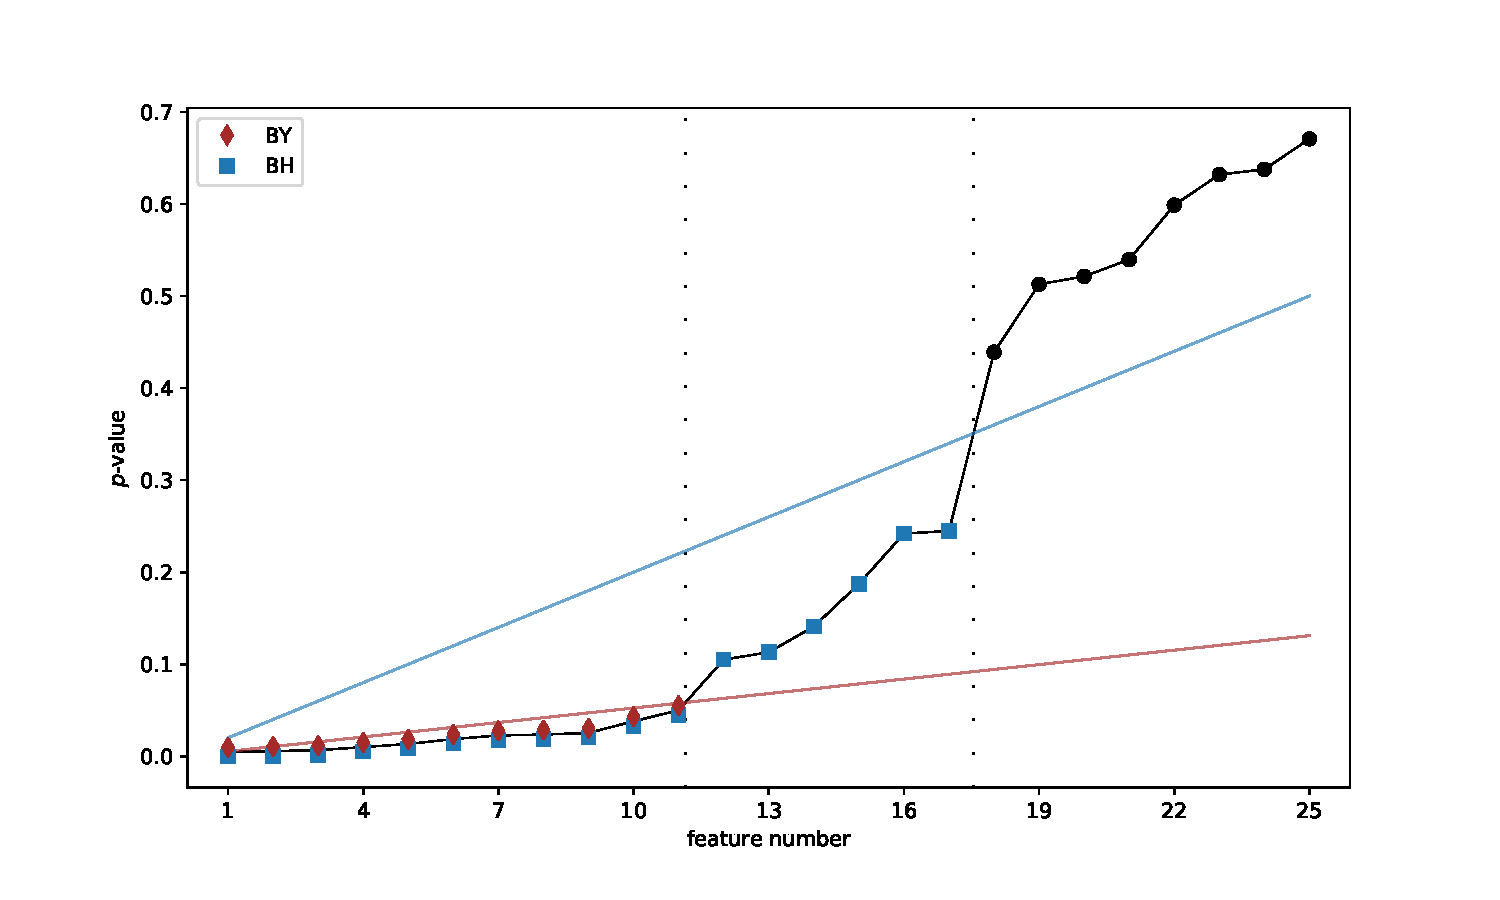
\includegraphics[width=1.\textwidth]{figures/bhy.pdf}
    \caption{
        Illustration of the BH and the BY procedures.
        Once the $p$-values are ordered,
        they are geometrically equivalent to drawing a line of slope $\beta$ going through the origin,
        identifying the last $p$-value under the line, and keeping features on its left.
        For BH, $\beta = \frac{\fdrtarget}{p}$ (in blue),
        while for BY, $\beta = \frac{\fdrtarget}{p \cdot c(p)}$ (in brown).
        In this toy example, $\fdrtarget = 0.5$, and it shows that BY is way more conservative than BH.
    }
    \label{fig:bhy}
\end{figure}
\bigbreak
Both procedures are illustrated in figure~\ref{fig:bhy}.
They require $p$-values to be computed, which is not always feasible, especially when $p > n$.
Furthermore, BH and BY have stronger guarantees than desired;
for a desired FDR level $\fdrtarget$,
they ensure that $\fdr \leq \frac{m_0}{p}\fdrtarget$,
and the factor $\frac{m_0}{p}$ might be much smaller than 1.

% \cite{statistical_inference_genome}\cite{resampled_fdr_control}\cite{unified_fdr_control}

    \chapter{The knockoffs filter framework}\label{ch:knockoffs}

Recently~\cite{fixed_x_knockoffs} introduced the knockoffs framework and extended it later in 2018 to a more general setting
(allowing in particular to perform feature selection in the high dimension context).
The goal is to control the false discovery rate as defined in Section~\ref{sec:fdrc},
while maintaining a reasonable power.
More formally, let $X \in \R^{n \times p}$ be a a feature matrix and $\yy \in \R^n$ the associated target vector.
Suppose $\yy$ depends only on the subset of features $\cS \subseteq \fset$.
Given some $\fdr$ target $\fdrtarget \in [0, 1]$, we wish to find a procedure such as, in average,
the false discovery proportion is smaller that $\fdrtarget$, i.e. $\fdr \leq q$.
To do so, the key idea is to construct for each original feature $X_j$, $j \in \fset$,
a knockoff (that is to say, fake) feature $\tX_j$ which is known to be out of the model.
Original features are then selected only if they prove to be more significant than their knockoff counterparts.

To compare a feature and its knockoff several quantities will be computed by interchanging matrix columns.
For this reason, we define the $\swap$ operator.
\begin{definition}\label{def:swap}
    \text{($\swap$ operator)}
    Given two matrices $A,\,B \in \R^{n \times p}$ of same size,
    we define the $\swap$ operator on the concatenated matrix $\big[ A,\, B \big]$ as follows.
    For a any subset of indices $S \subseteq \left\{ 1, \dots, p \right\}$,
    $\big[ A,\, B \big]_{\swap(S)}$ is the transformed matrix where the columns $A_j$ and $B_j$ were swapped for all
    $j \in S$.
\end{definition}

In the following sections, we are going to detail principal aspects of the construction of the knockoff features,
the computation of statistics for both original and knockoff features,
and the feature selection itself, based on those statistics.

\section{Knockoffs construction}\label{sec:kc}

In 2015, Barber-Candès introduced first the \textit{fixed}-X knockoffs variable selection procedure.
It relies on the creation of fake features satisfying some correlation constraints with the original features.
Unfortunately, it can only perform adequately when $n \geq 2p$,
even though it can be partially extended to the cases where $n \geq p$.
In 2018, Candès proposed an extension of the framework called \textit{model}-X knockoffs,
in which fake features are sampled from a learned distribution.
Despite the restriction of \textit{fixed}-X knockoffs, that method is still appealing as the construction of the
knockoff variables is straightforward (but costly).
On the other hand, \textit{model}-X knockoffs work in higher feature dimensions
but need an estimation of the distribution that generated the data,
which is a hard problem in general.
We will focus on the construction of \textit{model}-X knockoffs as we are principally interested in the
high dimensional setting.

In this section, let $(\cX, \cY)$ be a pair of random variables,
$\cX$ being composed of $p$ features,
and $\cY$ the associated target in $\R$.
We suppose that the feature matrix and the target vector $(X,\, \yy)$ are composed of samples from $(\cX,\, \cY)$.
We wish to build knockoff features $\tX \in \R^{n \times p}$, and to do so we are going to sample from a
random variable $\tcX$ built such that $\big[ \cX; \tcX \big]$
follows the properties~\ref{itm:cond_swap} and~\ref{itm:cond_indep} defined thereafter.

\subsection{General case}\label{subsec:general_case}

\begin{definition}
    \text{(model-$X$ knockoffs)}
    Given random vector $\cX \in \R^p$ of features,
    a random vector $\tcX \in \R^p$ is said to be model-$\cX$ knockoffs with respect to $\cY$
    if it satisfies the two following properties:
    \begin{enumerate}[label=\textbf{S.\arabic*},ref=S.\arabic*]
        \item \label{itm:cond_swap} For any $S \subseteq \fset$,
            $\big[ \cX; \tcX \big]^\top_{\swap(S)} \distreq \big[ \cX; \tcX \big]^\top$
        \item \label{itm:cond_indep} $\tcX \independent \cY \mid \cX$
    \end{enumerate}
\end{definition}
Intuitively, the condition~\ref{itm:cond_swap} ensures that a knockoff feature is sufficiently
close to its associated original feature so that swapping them doesn't change the distribution of the
concatenated random vector.
The independence condition~\ref{itm:cond_indep} states that the knockoff features
carry no additional information on $\cY$, given $\cX$.
It is trivially satisfied if $\tX$ is built without exploiting $\yy$.
However, constructing knockoffs meeting the first distribution equality is practically infeasible in general.
\begin{remark}
    Constructing the knockoffs feature matrix $\tX \in \R^{n \times p}$.
    It must satisfy two conditions, namely:
    \begin{align*}
        &{\tX}^\top\tX = \Sigma,
        \\
        &X^\top\tX = \Sigma - \diag\{\bs\}
        \text{ where } \bs \text{ is a non negative vector.}
    \end{align*}
    It ensures that $\tX$ has the same covariance as the original matrix $X$
    and that the correlation between distinct original and knockoff variables is
    the same as the correlation between the two originals.
\end{remark}

\subsection{Gaussian case}\label{subsec:gaussian_knockoffs}

In the particular case where $\cX$ is multivariate gaussian, the exact distribution of $\tcX$ can be derived.
\begin{proposition}
    \label{prop:gaussian_knockoffs}
    Suppose that $\cX \sim \cN(\bmu,\, \Sigma)$.
    If $\tcX$ is a random variable such that
    \begin{equation*}
        \big[ \cX; \tcX \big] \sim \cN\bigg(\begin{bmatrix} \bmu\\ \bmu \end{bmatrix},\, \Omega\bigg)
        ,\quad\text{where }\quad
        \Omega = \begin{bmatrix}
            \Sigma & \Sigma - \diag \bs\\
            \Sigma - \diag \bs & \Sigma
        \end{bmatrix}
        \quad\text{for some }
        \bs \in \R^p,
    \end{equation*}
    then $\big[\cX, \tcX \big]$ satisfies the $\swap$ property~\ref{itm:cond_swap},
    provided that $\Omega$ is positive semidefinite (so that it is indeed a covariance matrix).
\end{proposition}
In Proposition~\ref{prop:gaussian_knockoffs},
$\bs \in \R^p$ can be any vector such that $\Omega \succeq \0$.
We will come back later to the choice of $\bs$ which is actually crucial.
For now, assume that $\bs$ satisfies this assumption.
This result gives a way of constructing the knockoff features from $X$.
Indeed, as $\big[ \cX; \tcX \big]$ is multivariate normal, we may compute the exact distribution of
$\tcX \mid \cX$ with classical formulas~\cite{conditional_normal} as shown in~\ref{eq:conditional_gaussian_knockoffs}.
\begin{equation}\label{eq:conditional_gaussian_knockoffs}
    \tcX \mid \cX \sim \cN\left( \bupsilon,\, \Upsilon \right)
    ,\qquad\text{where}\quad
    \begin{cases*}
        \bupsilon = \cX - \cX\Sigma^{-1}\diag(\bs)\\
        \Upsilon = \diag(\bs)\left( 2I_{p \times p} - \Sigma^{-1}\diag(\bs) \right)
    \end{cases*}
\end{equation}
To put this into practice, one would compute the empirical mean
$\hat{\bmu} \in \R^p$ and covariance $\hat{\Sigma} \in \R^{p \times p}$ of $\cX$
using the observed feature matrix $X$.
Then, each row of $\tX$ is sampled according to a gaussian distribution $\cN\left( \bupsilon,\, \Upsilon \right)$
whose parameters are described in~\ref{eq:conditional_gaussian_knockoffs}.
Note in particular that the construction process is random;
if it is repeated, it may very well return different knockoffs, and thus different
selected features.
Because of this instability, several attempts~\cite{improve_stability_knockoffs} to fix it by
aggregating several knockoff samples.

Depending on the prior on the data and on the available computing power,
several algorithms may be used to estimate the covariance matrix $\Sigma$.
The empirical estimator is cheap but known to be unstable when $p > n$.
Shrunk estimations like Ledoit-Wolf~\cite{ledoit_wolf} provide good results.
\bigbreak
The gaussian hypothesis is obviously rarely verified in practice but yields acceptable results even when
$\cX$ is far from gaussian.
It partly comes from the fact that, rather than constructing $\tcX$ to respect~\ref{itm:cond_swap},
a weaker condition would be to enforce $\big[ \cX, \tcX \big]$ and $\big[ \cX, \tcX \big]_{\swap(S)}$ to have the
same first two moments (mean and covariance).
It turns out to be the case if $\tcX \mid \cX$ is constructed as described in~\ref{eq:conditional_gaussian_knockoffs}.
In the remaining of this master thesis, we will restrain ourselves to the gaussian hypothesis.

The first knockoff paper~\citep{fixed_x_knockoffs} introducing \textit{fixed}-X knockoffs relied on similar correlation
properties between the original and the knockoff features.
It however imposed $p \leq n$ and fewer statistics would yield theoretical guarantees regarding the FDR control
of the procedure.
In the reminding, we will only consider \textit{model}-X knockoffs as we are interested in the high dimensional
setting.
Moreover, \textit{model}-X knockoffs tend to give higher power experimentally compared to their \textit{fixed}
counterparts.

Note that generating knockoffs requires an estimation of the distribution of $\cX$ only,
and not $\cY \mid \cX$ as most methods would.
It is particularly appealing because labeling data is often the most costly part,
while acquiring samples $\xx \sim \cX$ is easier.
Unlabeled samples are thus valuable.

\section{Statistics computation}\label{sec:ksc}

\subsection{General principle}\label{subsec:scg}

Given the original feature matrix and the sampled knockoffs $X,\, \tX \in \R^{n \times p}$,
statistics $w_j$ for all $j \in \fset$ are computed.
Each $w_j$ represents how more significant the original feature $X_j$ is compared to $\tX_j$.
These statistics must satisfy the \emph{flip-sign} technical condition~\ref{def:flip_sign}
for the FDR control to carry out,
but a wide variety of choices is possible as will be shown.
\begin{definition}\label{def:flip_sign}
\text{(flip-sign property)}
A statistics function $\omega \colon \R^{n \times 2p} \times \R^n \to \R^p$
is said to follow the flip-sign property if for any $S \subseteq \fset$ and any $j \in \fset$,
\begin{equation*}
    \omega_j\big( \big[ X, \tX \big]_{\swap(S)},\, \yy \big) = \begin{cases*}
        -\omega_j\big( \big[ X, \tX \big],\, \yy \big) &\quad\text{if $j \in S$.}\\
        \omega_j\big( \big[ X, \tX \big],\, \yy \big) &\quad\text{otherwise.}
    \end{cases*}
\end{equation*}
\end{definition}
This property is very natural,
as it is simply asking the original and the knockoff features to play antisymmetric roles.

\subsection{Statistics aggregation}\label{subsec:ksa}

Constructing statistics satisfying the \emph{flip-sign} property~\ref{def:flip_sign} is actually straightforward
as an elementary scheme in two steps leads to such statistics.
The idea is to build statistics for each original and each knockoff feature, and then aggregate them.
\begin{enumerate}
    \item First construct statistics $[ \zz ; \tilde{\zz} ] = \zeta\big( \big[ X, \tX \big],\, \yy \big)$
        with some function $\zeta \colon \R^{n \times 2p} \times \R^n \to \R^{2p}$ satisfying
        \begin{equation}\label{eq:swap_cond}
        [ \zz ; \tilde{\zz} ]_{\swap(S)} = \zeta\big( \big[ X, \tX \big]_{\swap(S)},\, \yy \big)
        ,\quad
        \forall S \subseteq \fset
        \end{equation}
        The statistics $z_j$ (resp. $\tilde{z}_j$) indicates how significant the original (resp.\ knockoff) feature $j$ is.
    \item Then aggregate for each $j \in \fset$ the statistics of the original feature $z_j$ and the one of the corresponding
        knockoff $\tilde{z}_j$ with an antisymmetric function $a_j \colon \R\times\R \to \R$.
        That is, set $w_j = a_j(z_j, \tilde{z}_j)$.
\end{enumerate}
It is easy to show that such constructed statistics will satisfy the \emph{flip-sign} property~\ref{def:flip_sign}.

Basically any antisymmetric function $a_j$ could work, but some choices experimentally lead to a better power.
Here are a few examples of mappings:
\begin{itemize}
    \item $w_j = z_j - \tilde{z}_j$ (experimentally gives highest power in many cases)
    \item $w_j = \max(z_j, \tilde{z}_j) \times \sign(z_j - \tilde{z}_j)$ (first proposed in 2015)
    \item $w_j = \log\frac{z_j}{\tilde{z}_j}$
\end{itemize}
As for the function $\zeta$, it only needs to satisfy the \emph{swap} property~\ref{eq:swap_cond}.
This condition may seem restrictive but a large number of choices are actually valid.

\subsection{Examples}\label{subsec:sce}

A few examples of statistics relying on the aggregation trick are presented in this subsection.

In~\cite{fixed_x_knockoffs}, Barber-Candès suggest after empirical observations the use of the
Lasso Signed Max (LSM) statistics defined as follows.
\begin{equation}
    z_j = \sup\{\lambda \mid \hat{\bbeta}_j(\lambda) \neq 0\}
    ,\qquad\qquad
    \hat{\bbeta}(\lambda) =
    \underset{\bb}{\argmin}\;
    \frac{1}{2}\big\lVert \yy - \big[ X, \tX \big]\bb \big\rVert_2^2 + \lambda\norm{\bb}_1
\end{equation}
The vector $\hat{\bbeta}(\lambda) \in \R^{2p}$ contains the coefficients of a Lasso model
with penalty coefficient $\lambda > 0$.
As mentioned in subsection~\ref{subsubsec:lasso},
all the coefficients are null starting from $\lambda = +\infty$,
and are likely to shift (and to grow in absolute value) as $\lambda \to 0$.
It makes sense to use the first point where the coefficient $\beta_j$ is not null
as a significance metric for each individual feature $j$.
In addition, the LARS algorithms is able to compute that value pretty efficiently~\cite{lars_complexity}.

Training a plain Lasso estimator.
Once again, the LARS algorithm allows to cross-validate the Lasso efficiently.
Experimentally, the Lasso gives remarkable results in terms of power.

More generally, the coefficients in absolute value of any reasonable regressor
(or classifier, depending on the task) constitute a judicious option of statistics.
The fact that the \emph{flip-sign} property isn't restrictive makes the knockoff framework very powerful.
Depending on the data, an adapted model can be trained be it logistic regression,
SVMs, or random forests~\cite{random_forests}.
When the model has hyper-parameters, those are typically tuned using cross-validation.
This step is usually costly.

\section{Selection thresholds}\label{sec:kfs}

The selection itself requires the computation of a data-dependent threshold $\tau$
conditioned by the target FDR $\fdrtarget \in \zoint$.%, as defined in~\ref{eq:knock_thres} and~\ref{eq:knockp_thres}.
Finally, only the features $j$ whose statistics $w_j$ is above the threshold are selected.
\begin{equation}
    \hat{\cS} = \left\{ j \mid w_j \geq \tau \right\}
\end{equation}
Depending on how restrictive the procedure ought to be, the threshold $\tau$ can be adapted.
It leads to different guarantees regarding the control of the FDR\@.
Barber-Candès establish two selection procedures,
namely \emph{knockoff} and \emph{knockoff+}.
They control the modified FDR (as defined below) and the FDR respectively.
\begin{definition}\label{def:mfdr}
Given an estimate $\hat{\cS}$ of $\cS$ and a desired target false discovery rate $q \in [0, 1]$,
we define the modified $\fdr$ as follows:
\begin{equation*}
    \mfdr = \E{
        \frac
            {\abs{\left\{ j \mid j \in \hat{\cS} \setminus \cS \right\}}}
            {\lvert\hat{\cS}\rvert + 1 / q}
    }
\end{equation*}
\end{definition}
As $0 \leq q \leq 1$, $\mfdr$ as defined in~\ref{def:mfdr} is always smaller than the actual $\fdr$.
It means that controlling the $\mfdr$ is less restrictive than controlling the $\fdr$,
as the $\fdr$ could potentially be arbitrarily larger than the $\mfdr$.
But if the target threshold $q$ is not too small, and if many features are selected by the procedure,
the modified version of the FDR is close enough to the actual $\fdr$.
As will be shown later, being less restrictive by controlling only the $\mfdr$ can greatly improve the power
of the selection.

The only difference between the \emph{knockoff} and the \emph{knockoff+} procedures is the selection threshold $\tau$.
\begin{definition}
    (knockoff and knockoff+ thresholds)
    Given the statistics $\ww \in \R^p$ computed from $X$ and $\tX$,
    we define the knockoff and knockoff+ threshold respectively as follows:
    \begin{align}
        \tau &=
        \min\left\{
            t > 0 \mid \frac
                { \abs{\left\{ j \mid w_j \leq -t \right\}} }
                { \abs{\left\{ j \mid w_j \geq t \right\}} }
            \leq q
        \right\}\label{eq:knock_thres}\\
        \tau^+ &=
        \min\left\{
            t > 0 \mid \frac
                { 1 + \abs{\left\{ j \mid w_j \leq -t \right\}} }
                { \abs{\left\{ j \mid w_j \geq t \right\}} }
            \leq q
        \right\}\label{eq:knockp_thres}
    \end{align}
\end{definition}
They only differ by their numerator, where $\tau^+$ has an additional $+1$.
The main result of Barber-Candès regarding the control of the $\mfdr$ and $\fdr$ is stated in~\ref{th:knockoffs}.
\begin{theorem}\label{th:knockoffs}
    (guarantees of the knockoff procedures)
    Construct $\hat{\cS} = \left\{ j \mid w_j \geq \tau \right\}$
    and $\hat{\cS}^+ = \left\{ j \mid w_j \geq \tau^+ \right\}$.
    These selections ensure the following FDR controls:
    \begin{equation}
        \mfdr\big[ \hat{\cS} \big] \leq q
        ,\qquad
        \fdr\big[ \hat{\cS}^+ \big] \leq q
    \end{equation}
\end{theorem}
Even if only the \textit{knockoff+} method truly control the FDR,
using the threshold $\tau$ improves the power and gives reasonable FDR,
in the same way the BH procedure usually controls the FDR even when the tests are not independent.

\section{Bottlenecks}\label{sec:kb}

Despite the nice theoretical guarantees on the $\fdr$ control that the knockoff procedure proposes,
two bottlenecks hurt its performances in the high dimensional setting.

\subsection{SDP}\label{subsec:bot_sdp}

In the gaussian setting,
knockoff features are sampled according to the distribution~\ref{eq:conditional_gaussian_knockoffs}.
The control guarantees hold for any $\bs \in \R^p$ such that the covariance matrix $\Omega$ is semidefinite positive.
\begin{proposition}\label{prop:omega_psd}
    Let $\Omega = \begin{bmatrix}
        \Sigma & \Sigma - \diag \bs\\
        \Sigma - \diag \bs & \Sigma
    \end{bmatrix}$.
    Then $\Omega \succeq \0_{p \times p}$ if and only if $2\Sigma \succeq \diag \bs \succeq \0$.
\end{proposition}
\begin{proof}
    Note $D = \diag\bs$.
    By computing the Schur complement~\cite{schur_complement}
    $\Omega_{/\Sigma} = 2D - D\Sigma^{-1}D$,
    $\Omega \succeq \0$ is equivalent to $\Omega_{/\Sigma} \succeq \0$.
    Define $M$ and its Schur complements as follows
    \begin{equation*}
        M = \begin{bmatrix}
            2D & D\\
            D & \Sigma
        \end{bmatrix}
        ,\qquad\qquad
        \begin{cases*}
            M_{/2D} = \Sigma - \frac{1}{2}D\\
            M_{/\Sigma} = 2D - D\Sigma^{-1}D
        \end{cases*}
    \end{equation*}
    Finally, $\Omega_{/\Sigma} = M_{/\Sigma}$ is p.s.d.\ if and only if both $\Sigma - \frac{1}{2}D$ and $D$ are p.s.d.
\end{proof}
The FDR control holds for \emph{any} $\bs$ satisfying this constraint,
but some solutions lead to a better statistical power.
As will be shown in Chapter~\ref{ch:sdp},
finding good solutions amounts to solving a SDP which becomes intractable when $p$ is large.

\subsection{Statistics computation}\label{subsec:bot_stats}

and could take advantage of sparse naive Bayes to run faster.
\bigbreak
These two bottlenecks make the .
The following chapters tackle these two issues by proposing fast statistics computation.
From now, only binary classification problems will be considered, where the label $y$ takes values
in $\left\{ \cC^+,\, \cC^- \right\}$.

\section{Python implementation}\label{sec:python_implementation}

Barber-Candès (along with other coauthors) provided R and MATLAB implementations
of the knockoff framework\footnote{
    The R package page can be found at
    \href{https://cran.r-project.org/web/packages/knockoff/index.html}{this address}.
    Sources for both R and MATLAB are stored in this
    \href{https://github.com/msesia/knockoff-filter}{GitHub repository}.
}.
To the best of our knowledge, no public and unified Python implementation is presently available.
As Python is a very popular language in the machine learning community,
and as it keeps growing year after year,
we decided to make a Python implementation that contains fundamental components and that may be extended
depending on the needs\footnote{
    The implementation can be found at
    \href{}{this address}
}.
The implementation is deliberately compatible with Scikit-Learn~\cite{sklearn} estimators and .
It provides 3 main components,
namely a knockoffs generator \code{KnockoffsGenerator},
statistics computations utility functions,
and a selector \code{BaseKnockoffsSelector}.
\code{KnockoffsGenerator} and \code{BaseKnockoffsSelector} subclass \code{BaseEstimator} and \code{TransformerMixin}
and \code{BaseEstimator} and \code{SelectorMixin} from Scikit-Learn respectively,
so they are compatible with the Scikit-Learn ecosystem.
\begin{calgorithm}
\begin{minted}[linenos]{python}
selector = SimpleKnockoffsSelector(
    GaussianXKnockoffs(),
    z_to_w_statistics(estimator_statistics(estimator=LassoCV())),
    alpha=0.2,
)

selector.fit(X, y)
print(f'Selected features: {selector.mask_}')
\end{minted}
\caption{
    Example of knockoffs usage
}\label{code:python_knockoffs}
\end{calgorithm}

\bigbreak
In the following chapters,
we present the ideas and algorithms that we implemented to make this Python toolkit scalable to large dimensions.

    \cleardoublepage
    \chapter{Sparse naive Bayes}\label{ch:snb}

Naive Bayes was first introduced in the early 60s by~\cite{original_naive_bayes} for text documents classification.
It is a simple model assuming the independence of the features, given the label.
Despite this naive presupposition,
naive Bayes remains an engaging model for large scale datasets because of its low complexity.
The time complexity to train a model is asymptotically $\cO\left( n \cdot p \right)$,
where $n$ and $p$ are the number of samples and the number of features respectively.
Another appealing propriety is that naive Bayes can be trained in an online fashion,
as new data points come in a sequential order.
It can be particularly helpful if the dataset doesn't fit in memory.
Furthermore, distributed implementations could even be considered in order to speed up the learning process.

In this chapter, classical naive Bayes along with a few notations are briefly introduced.
Then, a sparse version of naive Bayes is presented,
allowing in particular to perform feature selection.

\section{Reminders on vanilla naive Bayes}\label{sec:naive_bayes}

In this section, we recall briefly the naive Bayes model in the specific case of binary classification,
and some details regarding the training phase under the bernoulli, multinomial and gaussian underlying assumptions.
Most key results can naturally be extended to the multiple classes setting.

Let $n$ and $p$ be two integers, $X \in \R^{n \times p}$ a design matrix
and $\yy \in \bset^n$ the associated target vector.
The negative and the positive classes are noted $\cC_-$ and $\cC_+$ respectively,
and will be indifferently substituted with their respective labels.

\subsection{General settings}\label{subsec:nb_general}

Note $\left( \cX,\, \cY \right)$ the pair of random variables that generated the samples and targets $X$ and $\yy$.
The goal is to explain $\yy$ given $X$, that is, finding the posterior probabilities $\Pr(\cC_\pm \mid \cX)$.
Given these probabilities, a new observation $\xx \in \R^p$ is classified according to the highest
posterior probability between the two classes
\begin{equation}\label{eq:nb_inference}
    y\left( \xx \right) = \underset{\cC \in \bclasses}{\argmax} \Pr\left( \cC \mid \xx \right)
\end{equation}
To do so, we combine the use of Bayes rule and make the (very) naive assumption that
all the features are independent given the class, that is
\begin{equation}
    \Pr\left( \cX = \xx \mid \cC_\pm \right) = \prod_{j = 1}^p \Pr(\cX_j = x_j \mid \cC_\pm)
    ,\qquad
    \Pr(\cC_\pm \mid \cX = \xx) = \frac{\Pr(\cX = \xx \mid \cC_\pm) \cdot \Pr(\cC_\pm)}{\Pr(\cX = \xx)}
\end{equation}
On the right hand side,
the denominator $\Pr(\cX = \xx)$ does not depend on the class $\cC_\pm$.
It is therefore not required to evaluate it in order to perform the inference described in~\ref{eq:nb_inference}.
Thus, we only need to estimate the probabilities $\Pr(\cC_\pm)$ and $\Pr(\xx \mid \cC_\pm)$.
The former are simply data averages, i.e.\ the frequencies of the positive and negative classes in the observed data.
As for the latter probabilities $\Pr\left( \xx \mid \cC_\pm \right) = \prod_{j = 1}^p \Pr(x_j \mid \cC_\pm)$,
they can be modeled by a plethora of distribution families, depending on the prior knowledge we have on the data.
The distribution is typically parametrized by some vector $\btheta \in \R^m$.
The probabilities are usually computed by maximizing the likelihood $\cL$,
or equivalently the log-likelihood $\lglh = \log\cL$, of the observed data.
\begin{equation*}
    \lglh\left( \btheta \right) = \sum_{i = 1}^n \Pr\left( \xx_i \mid y_i \,; \btheta \right)
\end{equation*}
We present now 3 meaningful cases, where the prior distributions of $\Pr(\xx \mid \cC_\pm)$ are either
gaussian, bernoulli or multinomial.
Let $\cI_\pm = \left\{ i \in \pset \mid y_i = \cC_\pm \right\}$ be the sets containing the
indexes of the positive and negative data points.
We also note for each class $\cC_\pm$ their cardinalities and empirical sums respectively, as follows:
\begin{equation*}
    n^\pm = | \cI_\pm |,
    \qquad\qquad
    \ff^\pm = \sum_{i \in \cI_\pm} \xx_i
\end{equation*}

\subsection{Gaussian naive Bayes}\label{subsec:gnb}

In this case the observed data conditioned on its label is modeled by the gaussian distribution
$\cN( \bmu^\pm, \Sigma^\pm )$.
It is the most common configuration because it can account for continuous data and the normal distribution constitures
a decent prior in many cases by virtue of its high entropy.
Note that the covariances $\Sigma^\pm \in \R^{p \times p}$
are diagonal as a result of the independence assumption that we made.
\begin{equation*}
    \Pr\left( \xx \mid C_\pm \right) =
    \frac{1}{\sqrt{(2\pi)^p\det(\Sigma_\pm)}}
    \exp\left( -\frac{1}{2}(\xx - \bmu_\pm)^\top\Sigma^{-1}(\xx - \bmu_\pm) \right)
\end{equation*}
By denoting $\sigma_j = \Sigma_{j j}$, the log-likelihood can be written
\begin{equation*}
    \begin{split}
        \lglh_g\left( \bmu_+,\, \ssigma_+,\; \bmu_-,\, \ssigma_-\right ) &=
            \sum_{j = 1}^p \Bigg[
                \sum_{i \in \cI_+}
                    -\frac{1}{2} \log \left( 2\pi \right)
                    -\log \sigma_j^+
                    -\frac{(x_j - \mu^+_j)^2}{2{\sigma^+_j}^2}\\
                &\qquad\quad+ \sum_{i \in \cI_-}
                    -\frac{1}{2} \log \left( 2\pi \right)
                    -\log \sigma_j^-
                    -\frac{(x_j - \mu^-_j)^2}{2{\sigma^-_j}^2}
            \Bigg]
    \end{split}
\end{equation*}
Even if $\lglh_g$ is not concave, it maximizer admits a closed-form solution
(readily shown to be the point where the gradient is null)
\begin{align*}
    \bmu^\pm = \frac{\ff^\pm}{n^\pm}
    ,\qquad\quad
    \ssigma^\pm = \sqrt{\frac{1}{n^\pm} \sum_{i \in \cI^\pm} (\xx_i - \bmu^\pm)^2}
\end{align*}

\subsection{Bernoulli naive Bayes}\label{subsec:bnb}

The Bernoulli distribution assumes that the design matrix is binary,
that is $X \in \zoset^{n \times p}$.
Even though this situation isn't very prevalent in practice, it has a simple and elegant solution.
In order to model the conditional probabilities, we may assume the existence of
$\btheta^+,\, \btheta^- \in \left( 0, 1 \right)^p$
such that for any data point $\xx \in \R^p$,
\begin{equation*}
    \Pr\left( x_j \mid \cC_\pm \right) = (\theta^\pm_j)^{x_j} \cdot (1 - \theta^\pm_j)^{1 - x_j}
\end{equation*}
It yields that $\log \Pr\left( \xx \mid \cC_\pm \right) =
\xx^\top\log\btheta^\pm + (\1 - \xx)^\top\log\left( \1 - \btheta^\pm \right)$
and finally
\begin{align}\label{eq:bernoulli_snb_ll}
    \lglh_b\left( \btheta^+,\, \btheta^- \right)
    &= \sum_{i \in \cI^+} \log \Pr\left( \xx_i \mid \cC_+ \right)
        + \sum_{i \in \cI^-} \log \Pr\left( \xx_i \mid \cC_- \right)\nonumber\\
    \begin{split}
        &= \ff_+^\top\log\btheta^+ + (n_+\1 - \ff_+)^\top\log\left( \1 - \btheta^+ \right)\\
        &\qquad+ \ff_-^\top\log\btheta^- + (n_-\1 - \ff_-)^\top\log\left( \1 - \btheta^- \right)
    \end{split}
\end{align}
The independence assumption makes the optimization problem decomposable across features;
it reduces to $p$ simpler maximizations, each of them being concave and admitting a closed-form solution.
Finally, we find that
\begin{equation*}
    \theta_\pm^\star = \frac{f^\pm}{n^\pm}
    ,\qquad\qquad
    \text{which are simply the averages of each class.}
\end{equation*}

\subsection{Multinomial naive Bayes}\label{subsec:mnb}

Multinomial naive Bayes generalizes the Bernoulli version
as it supposes that $X \in \N^{n \times p}$ is generated by the following underlying distribution
\begin{equation}\label{eq:multinomial_pr}
    \Pr\left( \xx \mid \cC_\pm \right) =
        \frac{\big( \sum_{j = 1}^p x_j \big)!}
            {\prod_{j = 1}^p x_j!} \cdot \prod_{j = 1}^p (\theta^\pm_j)^{x_j}
\end{equation}
In the special case where $X \in \zoset^{n \times p}$ we recover the above Bernoulli formulation.
It is parametrized by $\btheta^+,\, \btheta^- \in \left( 0,\, 1 \right)^p$, and they must satisfy
$\1^\top\btheta^+ = \1^\top\btheta^- = 1$ for~\ref{eq:multinomial_pr} to be a proper distribution.
Note that this model is still valid in the more general case
where we only assume the data to be non-negative, $X \in \R_+^{n \times p}$.
Hence, it is not as restrictive as it may appear at first sight,
as it is applicable to a large number of datasets.
The log probability is given by
\begin{equation*}
    \log\Pr\left(\xx \mid \cC_\pm\right) =
        \xx^\top\log\btheta_\pm + \log\frac{\big(\sum_{j = 1}^p x_j\big)!}{\prod_{j = 1}^p x_j!}
\end{equation*}
and the log-likelihood reduces to (after removing the constant terms)
\begin{equation}\label{eq:multinomial_snb_ll}
    \lglh_m\left(\btheta^+,\, \btheta^-\right) = \ff_+^\top\log\btheta^+ + \ff_-^\top\log\btheta^-
\end{equation}
which is again decomposable across features.
It turns out that the optimums are
\begin{equation*}
    \btheta_\pm^\star = \frac{\ff^\pm}{\1^\top\ff^\pm}
\end{equation*}
\bigbreak
In the models presented above, the time complexity to train the naive Bayes classifier is $\cO(n \cdot p)$.
With a larger number of classes besides $\cC^-$ and $\cC^+$, say $k$ classes, this complexity is multiplied by $k$.
On top of this low asymptotic complexity,
the solutions can be computed in closed-form, which makes the effective computation cost very low.
In comparison, no closed-form solution exist for the Lasso, for logistic regression~\cite{logistic_regression},
and for SVMs~\cite{svm}.
These models are usually trained by employing more costly gradient-descent based algorithms to find the global optimum.

\subsection{Decision boundary}\label{subsec:nb_bound}

Given a new data point $\xx \in \R^p$, we wish to attribute it the most probable label
$y \in \left\{ \cC^-,\, \cC^+ \right\}$.
No matter what model parametrized by $\btheta$ was chosen,~\ref{eq:nb_inference} reduces to
\begin{align*}
    y &= \underset{\cC \in \bclasses}{\argmax} \Pr\left( \cC \mid \xx \right)\\
    &= \sign \log \frac{\Pr(\cC^+ \mid \xx \,;\,\btheta)}{\Pr(\cC^- \mid \xx \,;\,\btheta)}\\
    &= \sign\bigg[\log \frac{\Pr(\cC^+)}{\Pr(\cC^-)}
            + \log \frac{\Pr(\xx \mid \cC^+)}{\Pr(\xx \mid \cC^-)}\bigg]
\end{align*}
In the cases of \emph{bernoulli} (\ref{subsec:bnb}) and \emph{multinomial} (\ref{subsec:mnb}) naive Bayes,
there exist $v \in \R$ and $\ww \in \R^p$ such that $y = \sign(v + \ww^\top\xx)$.
In these two special cases, the decision boundary is a hyperplane (which doesn't happen for gaussian naive Bayes).
For both of them $v$ has the same value, and by noting $\ww_b$ and $\ww_m$ the weights for the bernoulli
and the multinomial case respectively, we have
\begin{equation*}
    v = \log\frac{\Pr(\cC^+)}{\Pr(\cC^-)}
    ,\qquad\quad
    \begin{cases*}
        \ww_b = \log(\btheta^+\odot(\1 - \btheta^-)) - \log(\btheta^-\odot(\1 - \btheta^+))\\
        \ww_m = \log\btheta^+ - \log\btheta^-
    \end{cases*}
\end{equation*}
The figure~\ref{fig:log_reg_nb_comparison} compares the decision boundary of logistic regression to the one
of gaussian naive Bayes.
\begin{figure}
    \centering
    \begin{subfigure}{.5\textwidth}
        \centering
        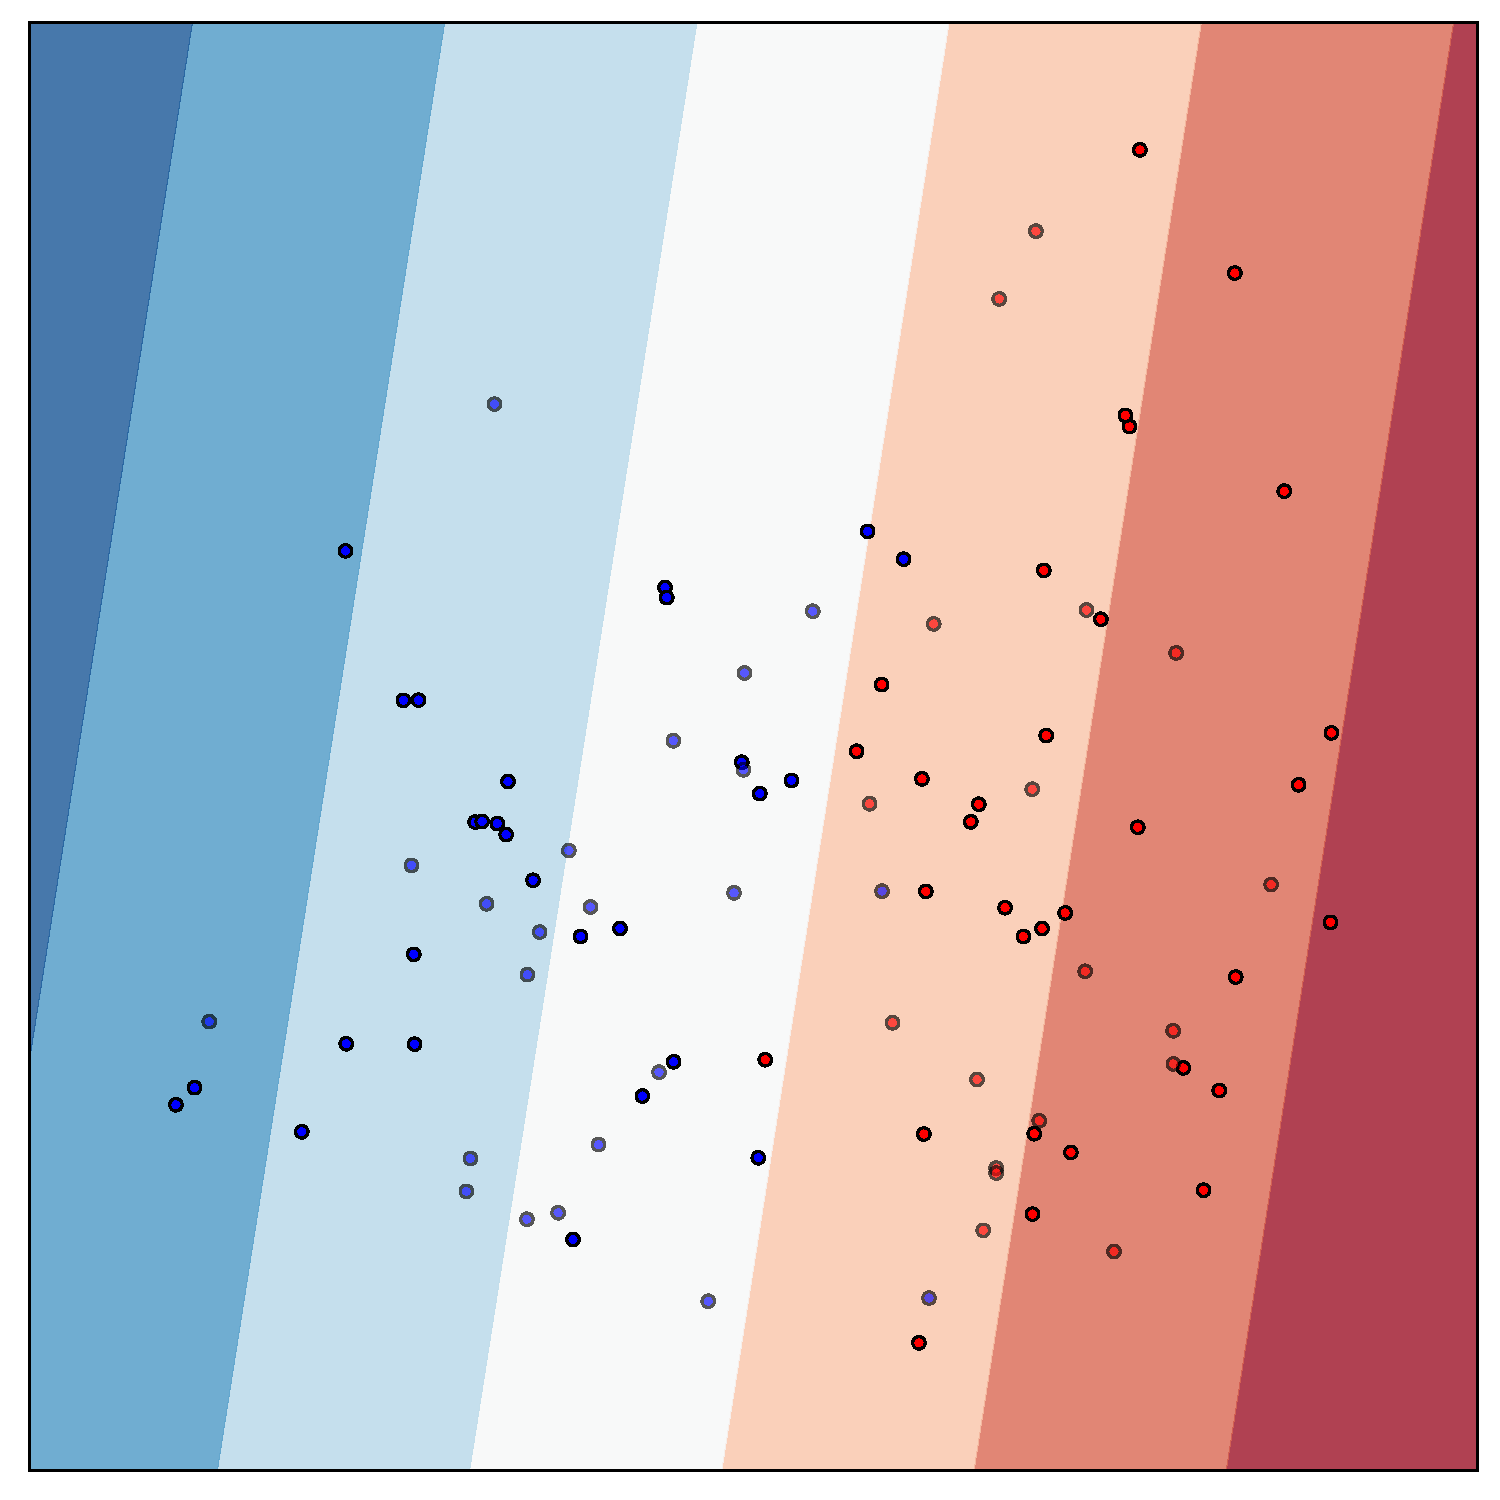
\includegraphics[width=0.75\linewidth]{figures/log_reg_classification.pdf}
        \label{fig:log_reg_classification}
    \end{subfigure}%
    \begin{subfigure}{.5\textwidth}
        \centering
        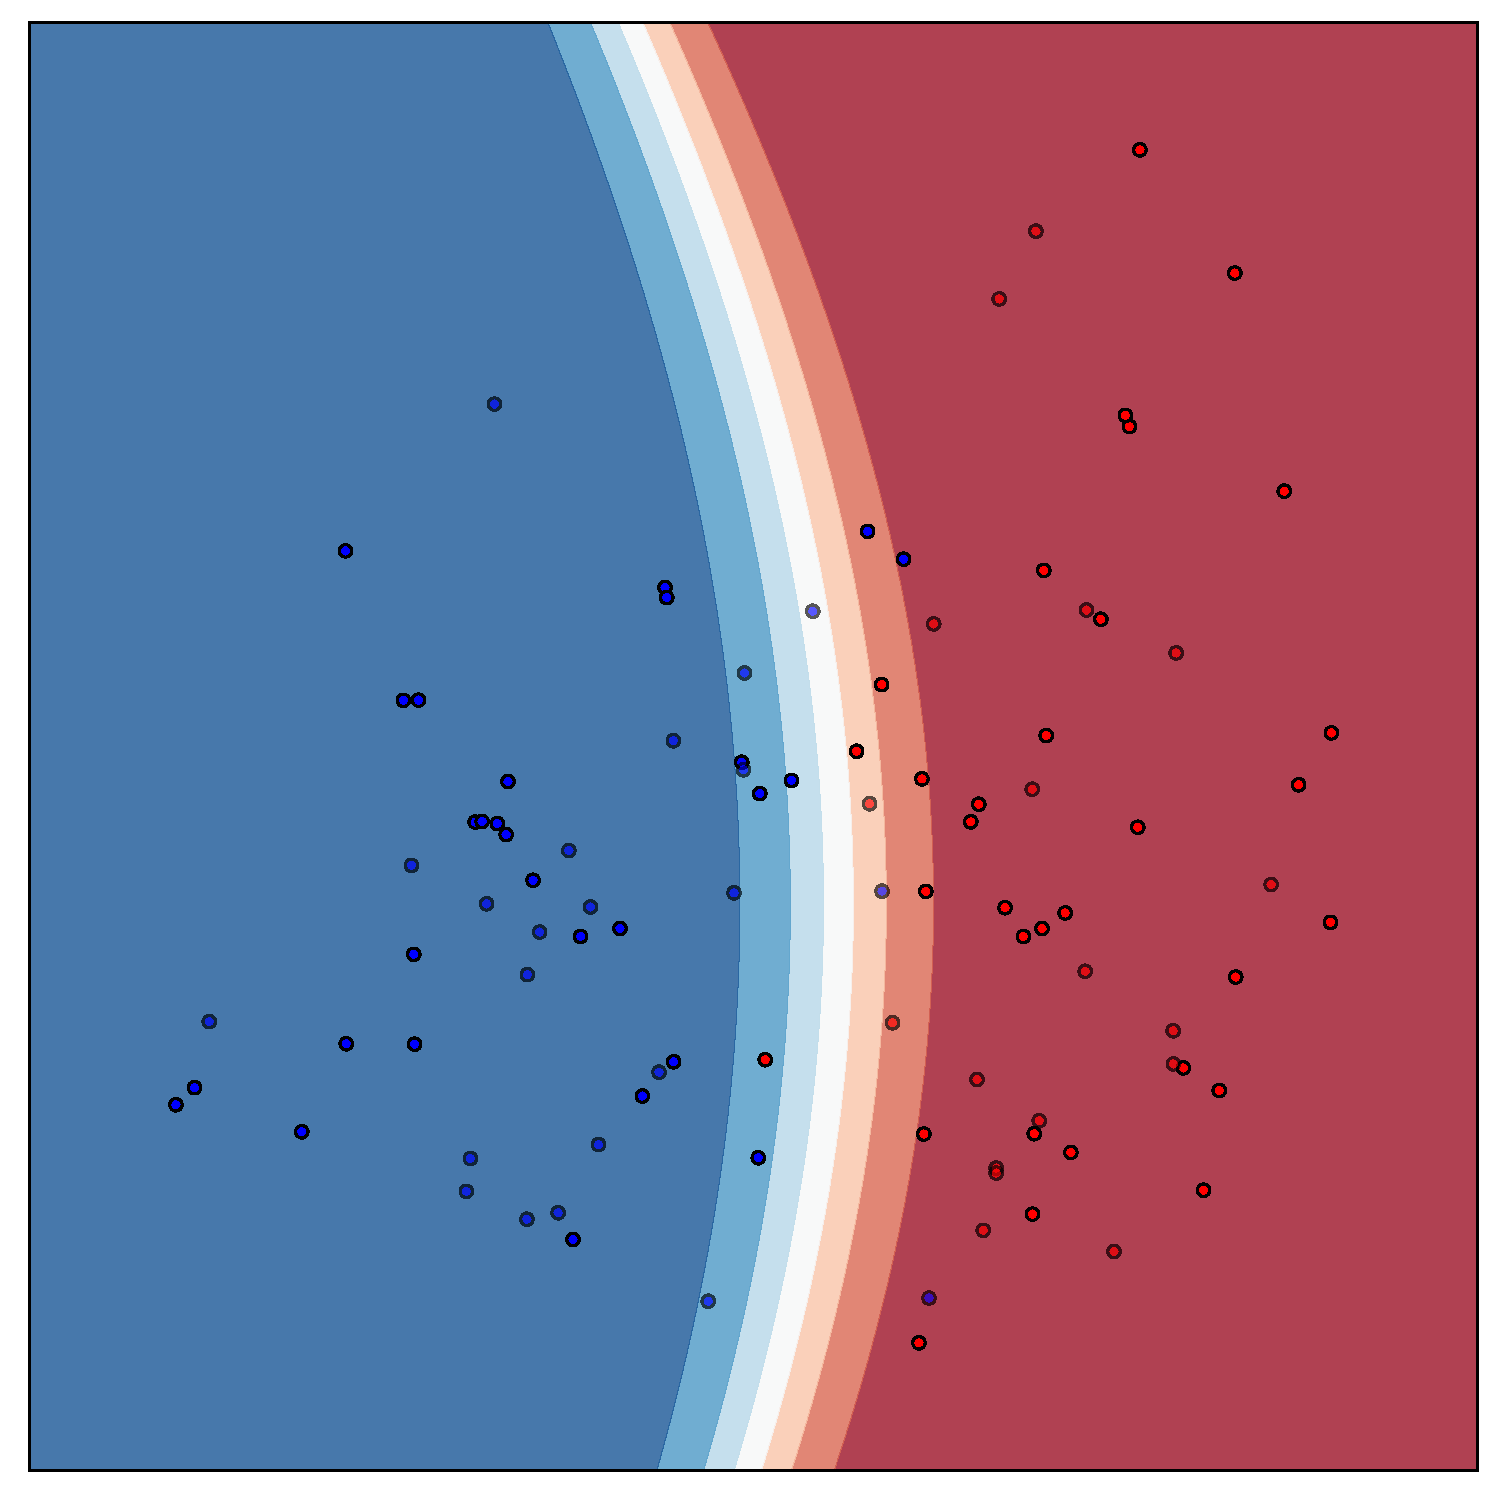
\includegraphics[width=0.75\linewidth]{figures/nb_classification.pdf}
        \label{fig:nb_classification}
    \end{subfigure}
    \caption{
        Illustration of the decision boundary for the logistic regression (left)
        and gaussian naive Bayes (right) for binary classification.
        For logistic regression, the separation is an hyperplane.
        For gaussian naive Bayes, the separation has a dependency on $x \odot x$ and can be non-linear.
        Both bernoulli and multinomial naive Bayes would have a linear separation.
    }
    \label{fig:log_reg_nb_comparison}
\end{figure}

\section{Sparse naive Bayes}\label{sec:snb}

A sparse version of naive Bayes was introduced in 2019~\cite{sparse_naive_bayes}.
They add a sparsity constraint in the Bernoulli and the multinomial optimization problems portrayed above.
It imposes the weight vector $\ww$ to have a number of non-zero entries under a certain threshold $k \in \N$.
That property is similar to the one of the Lasso presented in~\ref{subsubsec:lasso}.
But the sparsity in sparse naive Bayes (SNB) is controlled by an integer $k$ which is
the exact sparsity level desired on the weight vector,
while the Lasso relies on a continuous penalty coefficient $\lambda \in \R$.
This sparsity property makes SNB employable to perform feature selection,
by keeping only the features whose weights are non-zero.
Next sections detail the problem statement, the main results of the authors,
and some applications.

\subsection{Problem statement}\label{subsec:snb_ps}

Let $0 \leq k \leq p$ be a desired level of sparsity.
We wish to train a naive Bayes classifier whose decision boundary depends on at most $k$ features.
For any $\vv \in \R^d$ we note $\norm{\vv}_0$ the number of non-zero entries
(the cardinality) of the vector.
As shown in the previous section~\ref{subsec:nb_bound},
there exist $v \in \R$ and $\ww \in \R^p$ such that the prediction $y(\xx)$ for a new data point $\xx\in\R^p$ is
$\sign(v + \ww^\top\xx)$ for both bernoulli and multinomial naive Bayes.
Furthermore, the $j$th entry of the decision vector $\ww$ is null if and only if $\btheta^-_j = \btheta^+_j$,
where $\btheta^-$ and $\btheta^+$ are the parameters of the loss functions $\lglh_b$ and $\lglh_m$
in~\ref{eq:bernoulli_snb_ll} and~\ref{eq:multinomial_snb_ll} respectively.
Naturally, imposing the constraint $\norm{\btheta^+ - \btheta^-}_0 \leq k$ in the optimization problems
will yield a weight vector $\ww$ with the desired sparsity.
The optimization problems for Bernoulli and multinomial SNB
(shortened BSNB and MSNB respectively) can be phrased as follows:
\begin{equation}\label{eq:bsnb}\tag{BSNB}
    \begin{aligned}
        & \underset{\btheta^+,\, \btheta^-}{\text{maximize}}
        & & \lglh_\text{b}\left( \btheta^+,\, \btheta^- \right)
            \begin{split}
                &&&= \ff_+^\top\log\btheta^+ + (n_+\1 - \ff_+)^\top\log\left( \1 - \btheta^+ \right)\\
                &&&\qquad+ \ff_-^\top\log\btheta^- + (n_-\1 - \ff_-)^\top\log\left( \1 - \btheta^- \right)
            \end{split}\\
        & \text{subject to}
        & & \norm{\btheta^+ - \btheta^-}_0 \leq k.
    \end{aligned}
\end{equation}
\begin{equation}\label{eq:msnb}\tag{MSNB}
    \begin{aligned}
        & \underset{\btheta^+,\, \btheta^-}{\text{maximize}}
        & & \lglh_\text{m}\left( \btheta^+,\, \btheta^- \right) = \ff_+^\top\log\btheta^+ + \ff_-^\top\log\btheta^-\\
        & \text{subject to}
        & & \norm{\btheta^+ - \btheta^-}_0 \leq k\\
        & \text{ and }
        & & \1^\top\btheta^+ = \1^\top\btheta^- = 1.
    \end{aligned}
\end{equation}

\subsection{Main results and resolution}\label{subsec:snb_th}

Surprisingly and despite the combinatorial constraints,
these optimizations problems can be (approximately) solved very efficiently,
with an additional minor cost compared to vanilla naive Bayes.

Especially for the Bernoulli case,
an optimal solution can be computed in closed-form as shown in Theorem~\ref{th:bsnb}.
\begin{theorem}\label{th:bsnb}
    Suppose that $X \in \left\{ 0, 1 \right\}^{n \times p}$ is modeled by the Bernoulli distribution.
    Then, the exact solution to the problem~\ref{eq:bsnb} can be computed.
    First, define $\mt$ and $\uu$ as follows
    \begin{align*}
        \mt &= (\ff^+ + \ff^-) \odot \log\left( \frac{\ff^+ + \ff^-}{n} \right)
                + (n\1 - \ff^+ - \ff^-) \odot \log\left( \1 - \frac{\ff^+ + \ff^-}{n} \right)\\
        \begin{split}
                \uu &= \ff^+ \odot \log \frac{\ff^+}{n^+} + (n^+\1 - \ff^+) \odot \log (\1 - \frac{\ff^+}{n^+})\\
                &\qquad + \ff^- \odot \log \frac{\ff^-}{n^-} + (n^-\1 - \ff^-) \odot \log (\1 - \frac{\ff^-}{n^-})
        \end{split}
    \end{align*}
    Let $\cI$ be the set of $p - k$ smallest elements of $\uu - \mt$, and let
    \begin{equation*}
        {\theta^+_\star}_j = {\theta^-_\star}_j = \frac{1}{n}(f_j^+ + f_j^-)
        \;\forall j \in \cI
        ,\qquad
        {\theta^\pm_\star}_j = \frac{f^\pm_j}{n^\pm}
        \;\forall j \notin \cI
    \end{equation*}
\end{theorem}
Forming the vectors $\ff^-$ and $\ff^+$ is very quick
and takes asymptotically $\cO\left( n \cdot p \right)$ summations.
Then, constructing $\mt$ and $\uu$ can be done in $\cO\left( p \right)$ calculations.
Finding the $k$ largest elements of $\uu - \mt$ takes $\cO\left( p \cdot \log k \right)$ steps.
Finally, constituting $\btheta_\pm^\star$ requires $\cO\left( p \right)$ operations.
In total, the maximizer can be found in $\cO\left( n \cdot p + p \cdot \log k \right)$ steps,
which is very close to the cost $\cO\left( n \cdot p \right)$ of naive Bayes.

In the multinomial case, there is no closed-form solution, but a near-optimal one can be obtained as
stated in Theorem~\ref{th:msnb}.
\begin{theorem}\label{th:msnb}
    Suppose that $X \in \R_+^{n \times p}$ is modeled by the multinomial distribution.
    Then the dual of~\ref{eq:msnb} can be solved very efficiently and a good solution to the primal can be recovered.
    Define $\phi_k : \alpha \mapsto s_k(\hh(\alpha)) + C$ where $C$ is some constant,
    $s_k$ the sum of the k largest values of a vector, and
    \begin{equation*}
        \begin{split}
            \hh(\alpha) &= \ff_+ \odot \log \ff_+ + \ff_- \odot \log \ff_-
                    - (\ff_+ + \ff_-) \odot \log (\ff_+ + \ff_-)\\
                &\qquad - \ff_+ \log \alpha - \ff_- \log (1 - \alpha)
        \end{split}
    \end{equation*}
    $\phi_k$ is the dual of~\ref{eq:msnb} and can be minimized very quickly (with bisection for example)
    as it is a one-dimensional convex convex function.
    Let $\alpha^\star$ be its minimizer, $\cI$ the set of the $p - k$ smallest entries of
    $\hh(\alpha^\star)$, and $B_\pm = \sum_{j \notin \cI} f_i^\pm$.
    A primal point can be reconstructed as follows:
    \begin{equation*}
        {\theta^+_\star}_j = {\theta^-_\star}_j = \frac{f_j^+ + f_j^-}{\1^\top(\ff^+ + \ff^-)}
        \;\forall j \in \cI
        ,\qquad
        {\theta^\pm_\star}_j = \frac{B_+ + B_-}{B_\pm}\frac{f^\pm_j}{\1^\top(\ff^+ + \ff^-)}
        \;\forall j \notin \cI
    \end{equation*}
    Furthermore, it holds that $\psi(k - 4) \leq \phi(k) \leq \psi(k) \leq \phi(k + 4)$,
    implying that the duality gap is small if $\psi(k) - \psi(k - 4)$ is small.
\end{theorem}
Experimentally, the duality gap quickly converges to $0$ as $k$ increases,
and the reconstructed primal point is near-optimal.
The time complexity is once again $\cO(n \cdot p + p \cdot \log k)$,
which is a minor additional cost compared to plain naive Bayes.

The authors experiment SNB on several text datasets,
including AMZN, IMDB, TWTR, MPQA and SST2.
They compare it with more costly methods like the Lasso, $\ell_1$-penalized logistic regression and SVMs.
They obtain competitive test accuracies, while training their models several order of magnitude faster.

\section{Applications}\label{sec:nb_app}

The apparent low complexity of sparse naive Bayes compared to $\ell_1$-penalized methods such as
Lasso, logistic regression or SVMs makes is appealing for very large scale datasets.
We mention here a few applications to which we will come back later\footnote{
    An implementation of sparse naive Bayes can be found~\href{https://github.com/aspremon/NaiveFeatureSelection}{here}.
}.

\subsection{Criteo dataset}\label{subsec:snb_criteo}

As part of a Kaggle competition \emph{Display Advertising Challenge}\footnote{
    The Kaggle competition can be found at
    \href{https://www.kaggle.com/c/criteo-display-ad-challenge}{this address}.
}
in mid-2014, CriteoLabs shared log data collected over one week\footnote{
    The competition's dataset can be downloaded at
    \href{https://labs.criteo.com/2014/02/download-kaggle-display-advertising-challenge-dataset/}{this address}.
}
whose features were undisclosed for confidentiality purposes.
Main characteristics of this dataset can be found in Table~\ref{tab:criteo_dataset}.
\begin{table}[!htb]
    \centering
    \setlength{\tabcolsep}{2pt}
    {\small
    \begin{tabular}{|c|c|c|c|c|}\hline
    \textbf{Samples} & \textbf{Total features} & \textbf{Numerical features} & \textbf{Categorical features} & \textbf{Features after encoding}\\ \hline
    $45\,840\,617$ & $39$  & $13$ & $26$ & $33\,762\,590$ \\ \hline
    \end{tabular}
    }%
    \caption[short]{
        Criteo dataset characteristics.
        Even though the number of features is small,
        most categorical features have millions of categories.
        It makes the training of predicting models particularly challenging as it requires several
        dozens of GB of memory.
    }
    \label{tab:criteo_dataset}
\end{table}
It consists in $\approx 45$ millions of display ads with 39 features,
and a boolean label describing whether or not the ad was clicked by a customer.
Among these 39 features, 26 are categorical and a classical one-hot encoding would end up in millions of features.
This makes the Criteo dataset challenging, as it doesn't fit in the random-access memory after encoding,
and potentially not in the mass storage of a standard computer either.
Even on a small subset of the features, say 10\%,
selecting important features using Lasso or $\ell_1$-penalized logistic regression isn't realistic.
One-hot encoding isn't adapted to that situation.
Another approach would be to one-hot encode for each categorical feature only the most frequent categories,
and put the rest in a category \textit{other}.
The winners of the Kaggle competition used the hashing trick.
It consists in choosing an encoding space size $m$,
for example $m = 2^{20}$,
and defining some hash function $h \colon \text{Categories} \to \left\{ 0, \dots, m - 1 \right\}$.
This approach has several notable advantages.
First, the final encoded feature space $m$ can be adapted depending on the needs and on the computing power.
It may be used in an online fashion without a first pass
(that would be required for one-hot encoding in order to figure out all the existing categories).
Lastly, it naturally handles new labels in the test set that were unseen in the train set
(which would typically need a special \textit{other} category in the one-hot encoding setting).
Collisions between categories are likely to happen,
and even collisions between categories from different features.

We present here in Figure~\ref{fig:criteo_hash_elbow}.
$m = 2^{24} = 16777216$
All the computations are done on a standard workstation (16GB, Intel Core i7 3.60GHz $\times$ 8).
Sparse naive Bayes requires data averages to run,
i.e.\ the sums of the negative and of the positive points.
This part is time consuming but once these sums are computed they can be reused for any sparsity level $k$.
Using a light hash function and PyPy, they were obtained in around 20 minutes.
Only roughly half of the $2^{24}$ hash features were hit by the hash function.
Then, SNB optimum are computed for 1200 log-spaced points using a Python and NumPy implementation of SNB in 1 hour.
In this situation, what makes SNB particularly appealing is the fact that at no moment we need to load the full dataset
in memory.
We are only computing data averages whose shape are much smaller than the full matrix.
Note also that most tasks could even be distributed to speed up the computations.
\begin{figure}
    \centering
    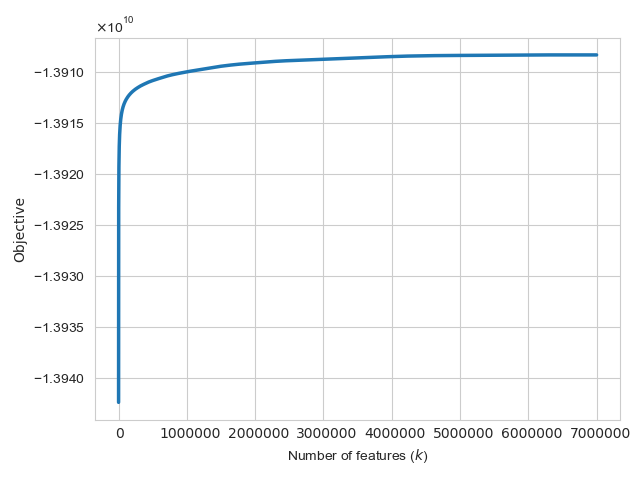
\includegraphics[width=0.75\linewidth, height=0.4\linewidth]{figures/criteo_hash_elbow.png}
    \caption{
        Optimal value of the~\ref{eq:msnb} optimization problem on the Criteo dataset
        as a function of the sparsity parameter $k$.
        Only 1--2 millions of the features explain most of the target vector (elbow heuristic).
    }
    \label{fig:criteo_hash_elbow}
\end{figure}

\bigbreak
Finally, sparse naive Bayes appear as an attractive alternative to the Lasso for the statistics computation
in the knockoff procedure~\ref{subsec:ksc}.

    \chapter{Fast statistics computation}\label{ch:fsc}

As described in Chapter~\ref{ch:knockoffs},
the computation of statistics on the concatenated feature matrix
is a key step of the knockoff selection process.
We discussed in Section~\ref{sec:ksc} the fact that a large variety of statistics control the FDR,
provided that the \textit{flip-sign} property~\ref{def:flip_sign} is satisfied.
However, the power is highly impacted depending on how suitable for the data the statistics are.

In this chapter, we note $X \in \R^{n \times p}$ the original design matrix,
and we suppose that we sampled valid knockoff features $\tX\in \R^{n \times p}$
(respecting conditions~\ref{itm:cond_swap} and~\ref{itm:cond_indep}).
The target vector is noted $\yy \in \R$.

\section{Lasso is good but slow}\label{sec:}

Experimentally, cross-validating a regressor (or classifier) against the data $\big[ X, \tX \big]$,
keeping its coefficients in absolute value,
and aggregating them as described in Subsection~\ref{subsec:ksa} yields excellent results.
Most classical regression models scale nicely as $p$ increases;
$\cO\left( n \cdot p \right)$ for Lasso~\citep{lasso} and logistic regression~\citep{logistic_regression},
$\cO\left( n \cdot p^2 \right)$ for support vector machines (SVM)~\citep{svm}.
In practice, the Lasso is observed to produce the highest statistical power in many cases~\citep{model_x_knockoffs}.
But all of these models have hyper-parameters that need to be tuned,
usually through cross-validation,
and with a naive grid search.
Tuning the estimator tends to lead to a higher power than picking ad hoc hyper-parameters,
but it increases the time complexity of the training phase by a lot.
Figure~\ref{fig:lasso_times} shows the time required to tune the penalty coefficient of a Lasso model,
using the algorithm LARS~\citep{lars}.
\begin{figure}
    \centering
    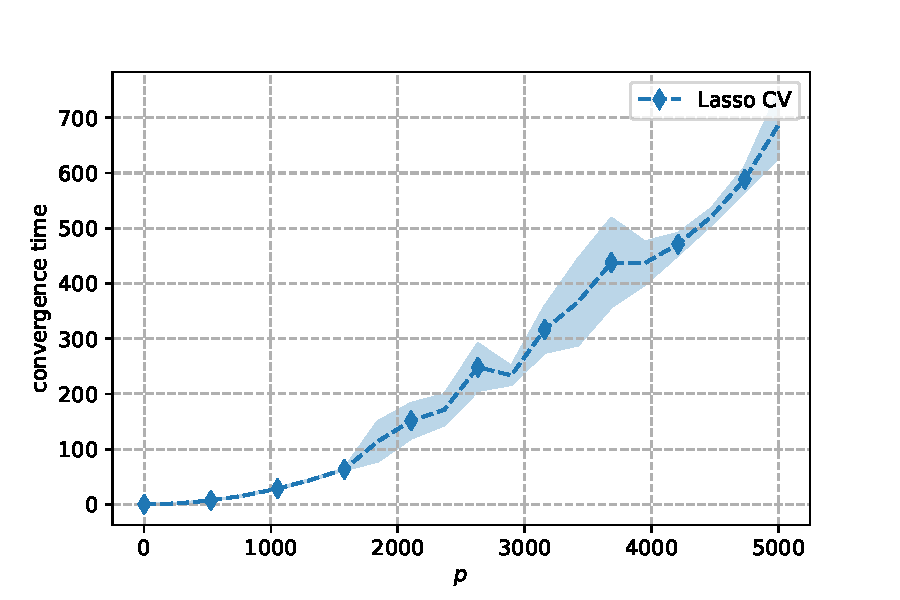
\includegraphics[width=0.8\linewidth, height=0.5\linewidth]{figures/lasso_cv_times.pdf}
    \caption{
        Convergence time (in seconds) to cross-validate the parameter $\lambda$ of a Lasso model,
        as a function of the feature space dimension $p$ (original + knockoff features).
        Benchmark done in Python using the class \code{LassoCV} from \code{sklearn.linear\_model}.
        The data is the one described in Section~\ref{sec:genetic_data},
        and contains $2\,695$ samples.
    }
    \label{fig:lasso_times}
\end{figure}
For $5\,000$ features (in total, with the knockoffs),
it already needs $\approx 12$ minutes to compute the statistics.

Many datasets, like the ones we will consider for experiments in Chapter~\ref{ch:exp},
contain dozens of thousands of features.
For this reason, we try to develop faster techniques and statistics in the following sections
(potentially at the cost of a lower power).

\section{Multi-stage procedures}\label{sec:multi_stage}

A natural way to address the high number of features is to split the selection into several steps.
If $p$ is high,
you may want to reduce the number of features by cutting
a large proportion of them with a cheap and fast procedure first
(for example univariate regression),
and use more sophisticated methods afterwards on the remaining set of features.
However, methods that control the FDR, like BH, BY, and the knockoffs, are not guaranteed to work with this
feature truncation approach anymore.
A modification of the BH procedure is proposed by~\cite{multi_stage_fdr}
to address the issue of this multi-stage evaluation.
They prove that their process effectively controls the FDR on the entire set of features, as desired.

In our Python implementation mentioned in Section~\ref{sec:python_implementation},
we propose a \code{MultiStepsSelector} class to do that kind of multi-steps selections.
We are well-aware that no theoretical guarantee exists in the case of the knockoff procedure.
But we observed on synthetic data that in practice the false discovery proportions obtained
were not too far away from the target value.
Making a theoretical analysis will be the subject of future work.

\section{Sparse naive Bayes}\label{sec:snb}

\chapter{Sparse naive Bayes}\label{ch:snb}

Naive Bayes was first introduced in the early 60s by~\cite{original_naive_bayes} for text documents classification.
It is a simple model assuming the independence of the features, given the label.
Despite this naive presupposition,
naive Bayes remains an engaging model for large scale datasets because of its low complexity.
The time complexity to train a model is asymptotically $\cO\left( n \cdot p \right)$,
where $n$ and $p$ are the number of samples and the number of features respectively.
Another appealing propriety is that naive Bayes can be trained in an online fashion,
as new data points come in a sequential order.
It can be particularly helpful if the dataset doesn't fit in memory.
Furthermore, distributed implementations could even be considered in order to speed up the learning process.

In this chapter, classical naive Bayes along with a few notations are briefly introduced.
Then, a sparse version of naive Bayes is presented,
allowing in particular to perform feature selection.

\section{Reminders on vanilla naive Bayes}\label{sec:naive_bayes}

In this section, we recall briefly the naive Bayes model in the specific case of binary classification,
and some details regarding the training phase under the bernoulli, multinomial and gaussian underlying assumptions.
Most key results can naturally be extended to the multiple classes setting.

Let $n$ and $p$ be two integers, $X \in \R^{n \times p}$ a design matrix
and $\yy \in \bset^n$ the associated target vector.
The negative and the positive classes are noted $\cC_-$ and $\cC_+$ respectively,
and will be indifferently substituted with their respective labels.

\subsection{General settings}\label{subsec:nb_general}

Note $\left( \cX,\, \cY \right)$ the pair of random variables that generated the samples and targets $X$ and $\yy$.
The goal is to explain $\yy$ given $X$, that is, finding the posterior probabilities $\Pr(\cC_\pm \mid \cX)$.
Given these probabilities, a new observation $\xx \in \R^p$ is classified according to the highest
posterior probability between the two classes
\begin{equation}\label{eq:nb_inference}
    y\left( \xx \right) = \underset{\cC \in \bclasses}{\argmax} \Pr\left( \cC \mid \xx \right)
\end{equation}
To do so, we combine the use of Bayes rule and make the (very) naive assumption that
all the features are independent given the class, that is
\begin{equation}
    \Pr\left( \cX = \xx \mid \cC_\pm \right) = \prod_{j = 1}^p \Pr(\cX_j = x_j \mid \cC_\pm)
    ,\qquad
    \Pr(\cC_\pm \mid \cX = \xx) = \frac{\Pr(\cX = \xx \mid \cC_\pm) \cdot \Pr(\cC_\pm)}{\Pr(\cX = \xx)}
\end{equation}
On the right hand side,
the denominator $\Pr(\cX = \xx)$ does not depend on the class $\cC_\pm$.
It is therefore not required to evaluate it in order to perform the inference described in~\ref{eq:nb_inference}.
Thus, we only need to estimate the probabilities $\Pr(\cC_\pm)$ and $\Pr(\xx \mid \cC_\pm)$.
The former are simply data averages, i.e.\ the frequencies of the positive and negative classes in the observed data.
As for the latter probabilities $\Pr\left( \xx \mid \cC_\pm \right) = \prod_{j = 1}^p \Pr(x_j \mid \cC_\pm)$,
they can be modeled by a plethora of distribution families, depending on the prior knowledge we have on the data.
The distribution is typically parametrized by some vector $\btheta \in \R^m$.
The probabilities are usually computed by maximizing the likelihood $\cL$,
or equivalently the log-likelihood $\lglh = \log\cL$, of the observed data.
\begin{equation*}
    \lglh\left( \btheta \right) = \sum_{i = 1}^n \Pr\left( \xx_i \mid y_i \,; \btheta \right)
\end{equation*}
We present now 3 meaningful cases, where the prior distributions of $\Pr(\xx \mid \cC_\pm)$ are either
gaussian, bernoulli or multinomial.
Let $\cI_\pm = \left\{ i \in \pset \mid y_i = \cC_\pm \right\}$ be the sets containing the
indexes of the positive and negative data points.
We also note for each class $\cC_\pm$ their cardinalities and empirical sums respectively, as follows:
\begin{equation*}
    n^\pm = | \cI_\pm |,
    \qquad\qquad
    \ff^\pm = \sum_{i \in \cI_\pm} \xx_i
\end{equation*}

\subsection{Gaussian naive Bayes}\label{subsec:gnb}

In this case the observed data conditioned on its label is modeled by the gaussian distribution
$\cN( \bmu^\pm, \Sigma^\pm )$.
It is the most common configuration because it can account for continuous data and the normal distribution constitures
a decent prior in many cases by virtue of its high entropy.
Note that the covariances $\Sigma^\pm \in \R^{p \times p}$
are diagonal as a result of the independence assumption that we made.
\begin{equation*}
    \Pr\left( \xx \mid C_\pm \right) =
    \frac{1}{\sqrt{(2\pi)^p\det(\Sigma_\pm)}}
    \exp\left( -\frac{1}{2}(\xx - \bmu_\pm)^\top\Sigma^{-1}(\xx - \bmu_\pm) \right)
\end{equation*}
By denoting $\sigma_j = \Sigma_{j j}$, the log-likelihood can be written
\begin{equation*}
    \begin{split}
        \lglh_g\left( \bmu_+,\, \ssigma_+,\; \bmu_-,\, \ssigma_-\right ) &=
            \sum_{j = 1}^p \Bigg[
                \sum_{i \in \cI_+}
                    -\frac{1}{2} \log \left( 2\pi \right)
                    -\log \sigma_j^+
                    -\frac{(x_j - \mu^+_j)^2}{2{\sigma^+_j}^2}\\
                &\qquad\quad+ \sum_{i \in \cI_-}
                    -\frac{1}{2} \log \left( 2\pi \right)
                    -\log \sigma_j^-
                    -\frac{(x_j - \mu^-_j)^2}{2{\sigma^-_j}^2}
            \Bigg]
    \end{split}
\end{equation*}
Even if $\lglh_g$ is not concave, it maximizer admits a closed-form solution
(readily shown to be the point where the gradient is null)
\begin{align*}
    \bmu^\pm = \frac{\ff^\pm}{n^\pm}
    ,\qquad\quad
    \ssigma^\pm = \sqrt{\frac{1}{n^\pm} \sum_{i \in \cI^\pm} (\xx_i - \bmu^\pm)^2}
\end{align*}

\subsection{Bernoulli naive Bayes}\label{subsec:bnb}

The Bernoulli distribution assumes that the design matrix is binary,
that is $X \in \zoset^{n \times p}$.
Even though this situation isn't very prevalent in practice, it has a simple and elegant solution.
In order to model the conditional probabilities, we may assume the existence of
$\btheta^+,\, \btheta^- \in \left( 0, 1 \right)^p$
such that for any data point $\xx \in \R^p$,
\begin{equation*}
    \Pr\left( x_j \mid \cC_\pm \right) = (\theta^\pm_j)^{x_j} \cdot (1 - \theta^\pm_j)^{1 - x_j}
\end{equation*}
It yields that $\log \Pr\left( \xx \mid \cC_\pm \right) =
\xx^\top\log\btheta^\pm + (\1 - \xx)^\top\log\left( \1 - \btheta^\pm \right)$
and finally
\begin{align}\label{eq:bernoulli_snb_ll}
    \lglh_b\left( \btheta^+,\, \btheta^- \right)
    &= \sum_{i \in \cI^+} \log \Pr\left( \xx_i \mid \cC_+ \right)
        + \sum_{i \in \cI^-} \log \Pr\left( \xx_i \mid \cC_- \right)\nonumber\\
    \begin{split}
        &= \ff_+^\top\log\btheta^+ + (n_+\1 - \ff_+)^\top\log\left( \1 - \btheta^+ \right)\\
        &\qquad+ \ff_-^\top\log\btheta^- + (n_-\1 - \ff_-)^\top\log\left( \1 - \btheta^- \right)
    \end{split}
\end{align}
The independence assumption makes the optimization problem decomposable across features;
it reduces to $p$ simpler maximizations, each of them being concave and admitting a closed-form solution.
Finally, we find that
\begin{equation*}
    \theta_\pm^\star = \frac{f^\pm}{n^\pm}
    ,\qquad\qquad
    \text{which are simply the averages of each class.}
\end{equation*}

\subsection{Multinomial naive Bayes}\label{subsec:mnb}

Multinomial naive Bayes generalizes the Bernoulli version
as it supposes that $X \in \N^{n \times p}$ is generated by the following underlying distribution
\begin{equation}\label{eq:multinomial_pr}
    \Pr\left( \xx \mid \cC_\pm \right) =
        \frac{\big( \sum_{j = 1}^p x_j \big)!}
            {\prod_{j = 1}^p x_j!} \cdot \prod_{j = 1}^p (\theta^\pm_j)^{x_j}
\end{equation}
In the special case where $X \in \zoset^{n \times p}$ we recover the above Bernoulli formulation.
It is parametrized by $\btheta^+,\, \btheta^- \in \left( 0,\, 1 \right)^p$, and they must satisfy
$\1^\top\btheta^+ = \1^\top\btheta^- = 1$ for~\ref{eq:multinomial_pr} to be a proper distribution.
Note that this model is still valid in the more general case
where we only assume the data to be non-negative, $X \in \R_+^{n \times p}$.
Hence, it is not as restrictive as it may appear at first sight,
as it is applicable to a large number of datasets.
The log probability is given by
\begin{equation*}
    \log\Pr\left(\xx \mid \cC_\pm\right) =
        \xx^\top\log\btheta_\pm + \log\frac{\big(\sum_{j = 1}^p x_j\big)!}{\prod_{j = 1}^p x_j!}
\end{equation*}
and the log-likelihood reduces to (after removing the constant terms)
\begin{equation}\label{eq:multinomial_snb_ll}
    \lglh_m\left(\btheta^+,\, \btheta^-\right) = \ff_+^\top\log\btheta^+ + \ff_-^\top\log\btheta^-
\end{equation}
which is again decomposable across features.
It turns out that the optimums are
\begin{equation*}
    \btheta_\pm^\star = \frac{\ff^\pm}{\1^\top\ff^\pm}
\end{equation*}
\bigbreak
In the models presented above, the time complexity to train the naive Bayes classifier is $\cO(n \cdot p)$.
With a larger number of classes besides $\cC^-$ and $\cC^+$, say $k$ classes, this complexity is multiplied by $k$.
On top of this low asymptotic complexity,
the solutions can be computed in closed-form, which makes the effective computation cost very low.
In comparison, no closed-form solution exist for the Lasso, for logistic regression~\cite{logistic_regression},
and for SVMs~\cite{svm}.
These models are usually trained by employing more costly gradient-descent based algorithms to find the global optimum.

\subsection{Decision boundary}\label{subsec:nb_bound}

Given a new data point $\xx \in \R^p$, we wish to attribute it the most probable label
$y \in \left\{ \cC^-,\, \cC^+ \right\}$.
No matter what model parametrized by $\btheta$ was chosen,~\ref{eq:nb_inference} reduces to
\begin{align*}
    y &= \underset{\cC \in \bclasses}{\argmax} \Pr\left( \cC \mid \xx \right)\\
    &= \sign \log \frac{\Pr(\cC^+ \mid \xx \,;\,\btheta)}{\Pr(\cC^- \mid \xx \,;\,\btheta)}\\
    &= \sign\bigg[\log \frac{\Pr(\cC^+)}{\Pr(\cC^-)}
            + \log \frac{\Pr(\xx \mid \cC^+)}{\Pr(\xx \mid \cC^-)}\bigg]
\end{align*}
In the cases of \emph{bernoulli} (\ref{subsec:bnb}) and \emph{multinomial} (\ref{subsec:mnb}) naive Bayes,
there exist $v \in \R$ and $\ww \in \R^p$ such that $y = \sign(v + \ww^\top\xx)$.
In these two special cases, the decision boundary is a hyperplane (which doesn't happen for gaussian naive Bayes).
For both of them $v$ has the same value, and by noting $\ww_b$ and $\ww_m$ the weights for the bernoulli
and the multinomial case respectively, we have
\begin{equation*}
    v = \log\frac{\Pr(\cC^+)}{\Pr(\cC^-)}
    ,\qquad\quad
    \begin{cases*}
        \ww_b = \log(\btheta^+\odot(\1 - \btheta^-)) - \log(\btheta^-\odot(\1 - \btheta^+))\\
        \ww_m = \log\btheta^+ - \log\btheta^-
    \end{cases*}
\end{equation*}
The figure~\ref{fig:log_reg_nb_comparison} compares the decision boundary of logistic regression to the one
of gaussian naive Bayes.
\begin{figure}
    \centering
    \begin{subfigure}{.5\textwidth}
        \centering
        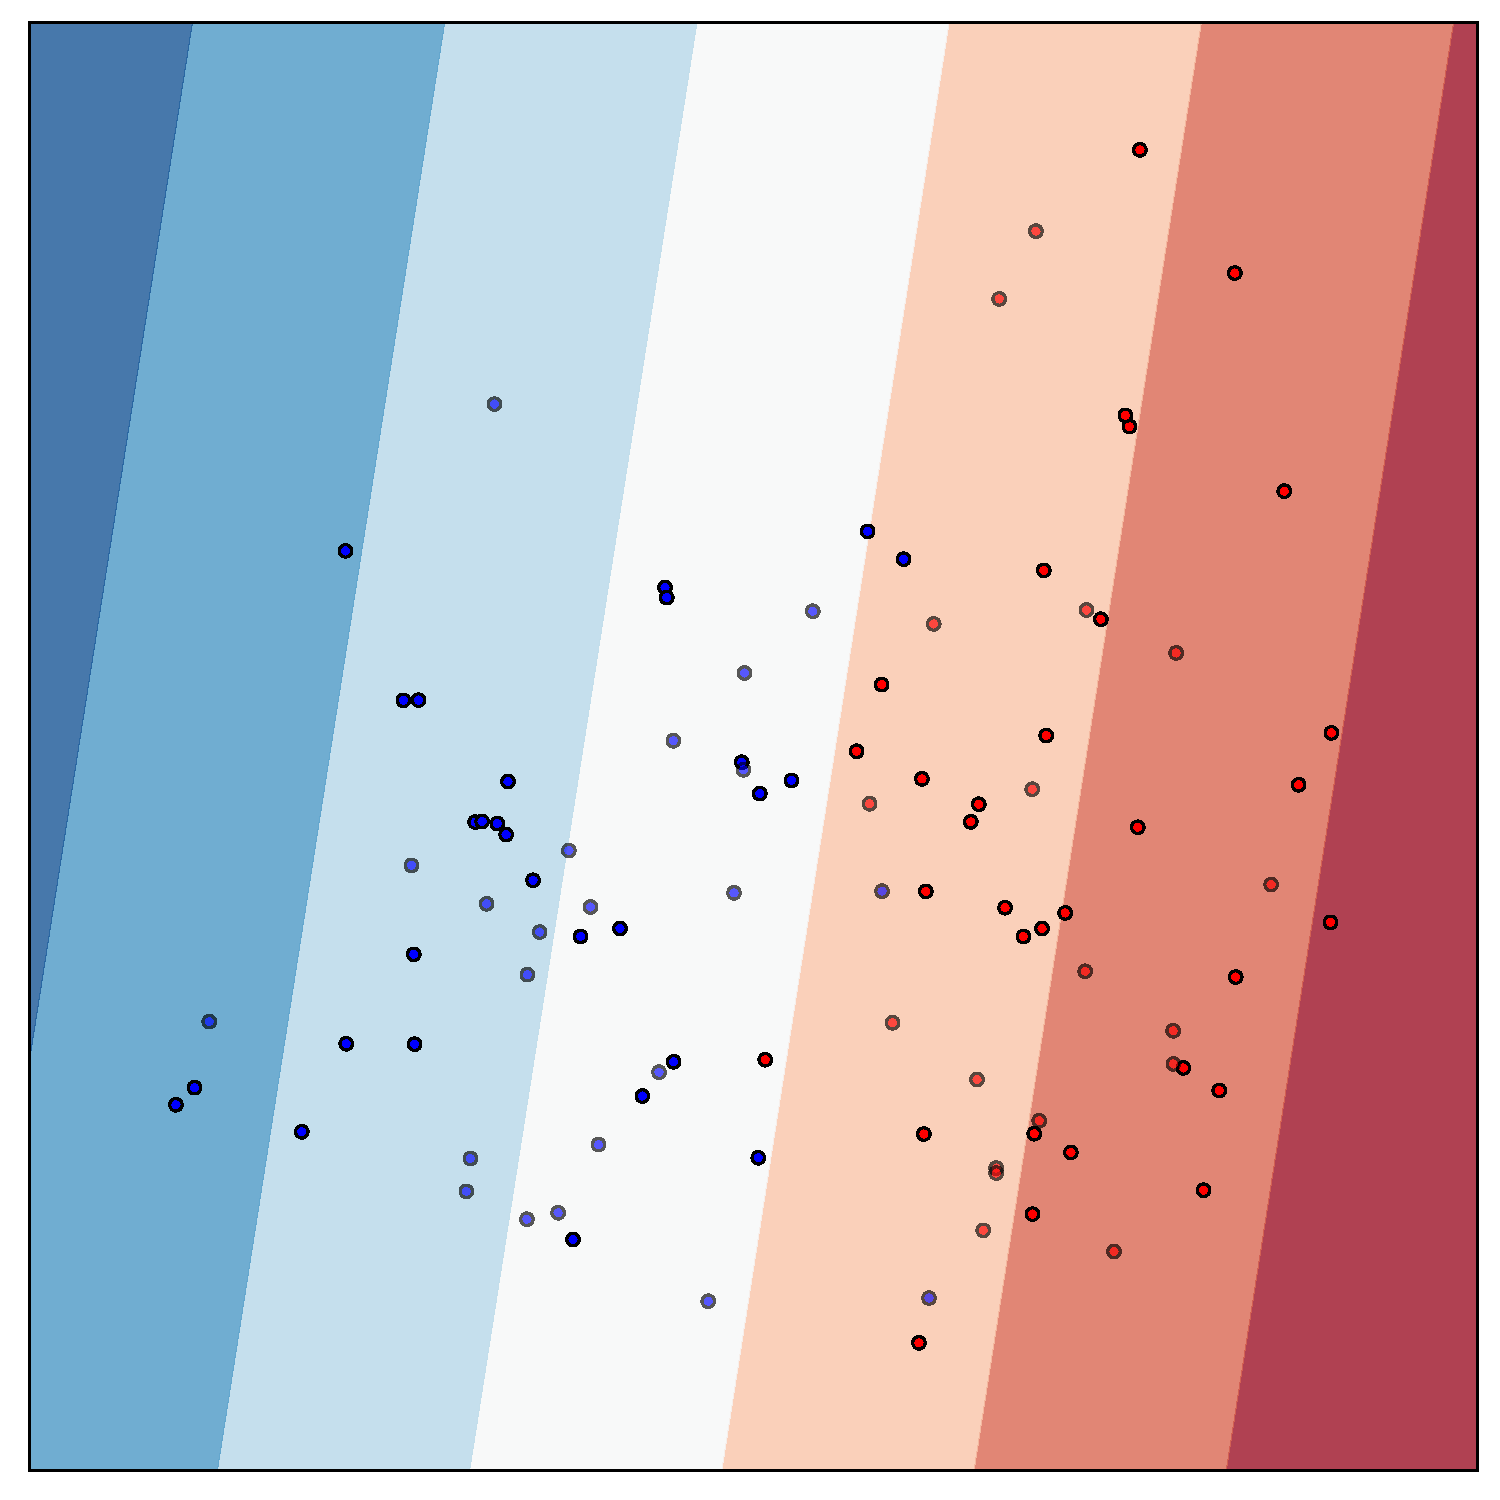
\includegraphics[width=0.75\linewidth]{figures/log_reg_classification.pdf}
        \label{fig:log_reg_classification}
    \end{subfigure}%
    \begin{subfigure}{.5\textwidth}
        \centering
        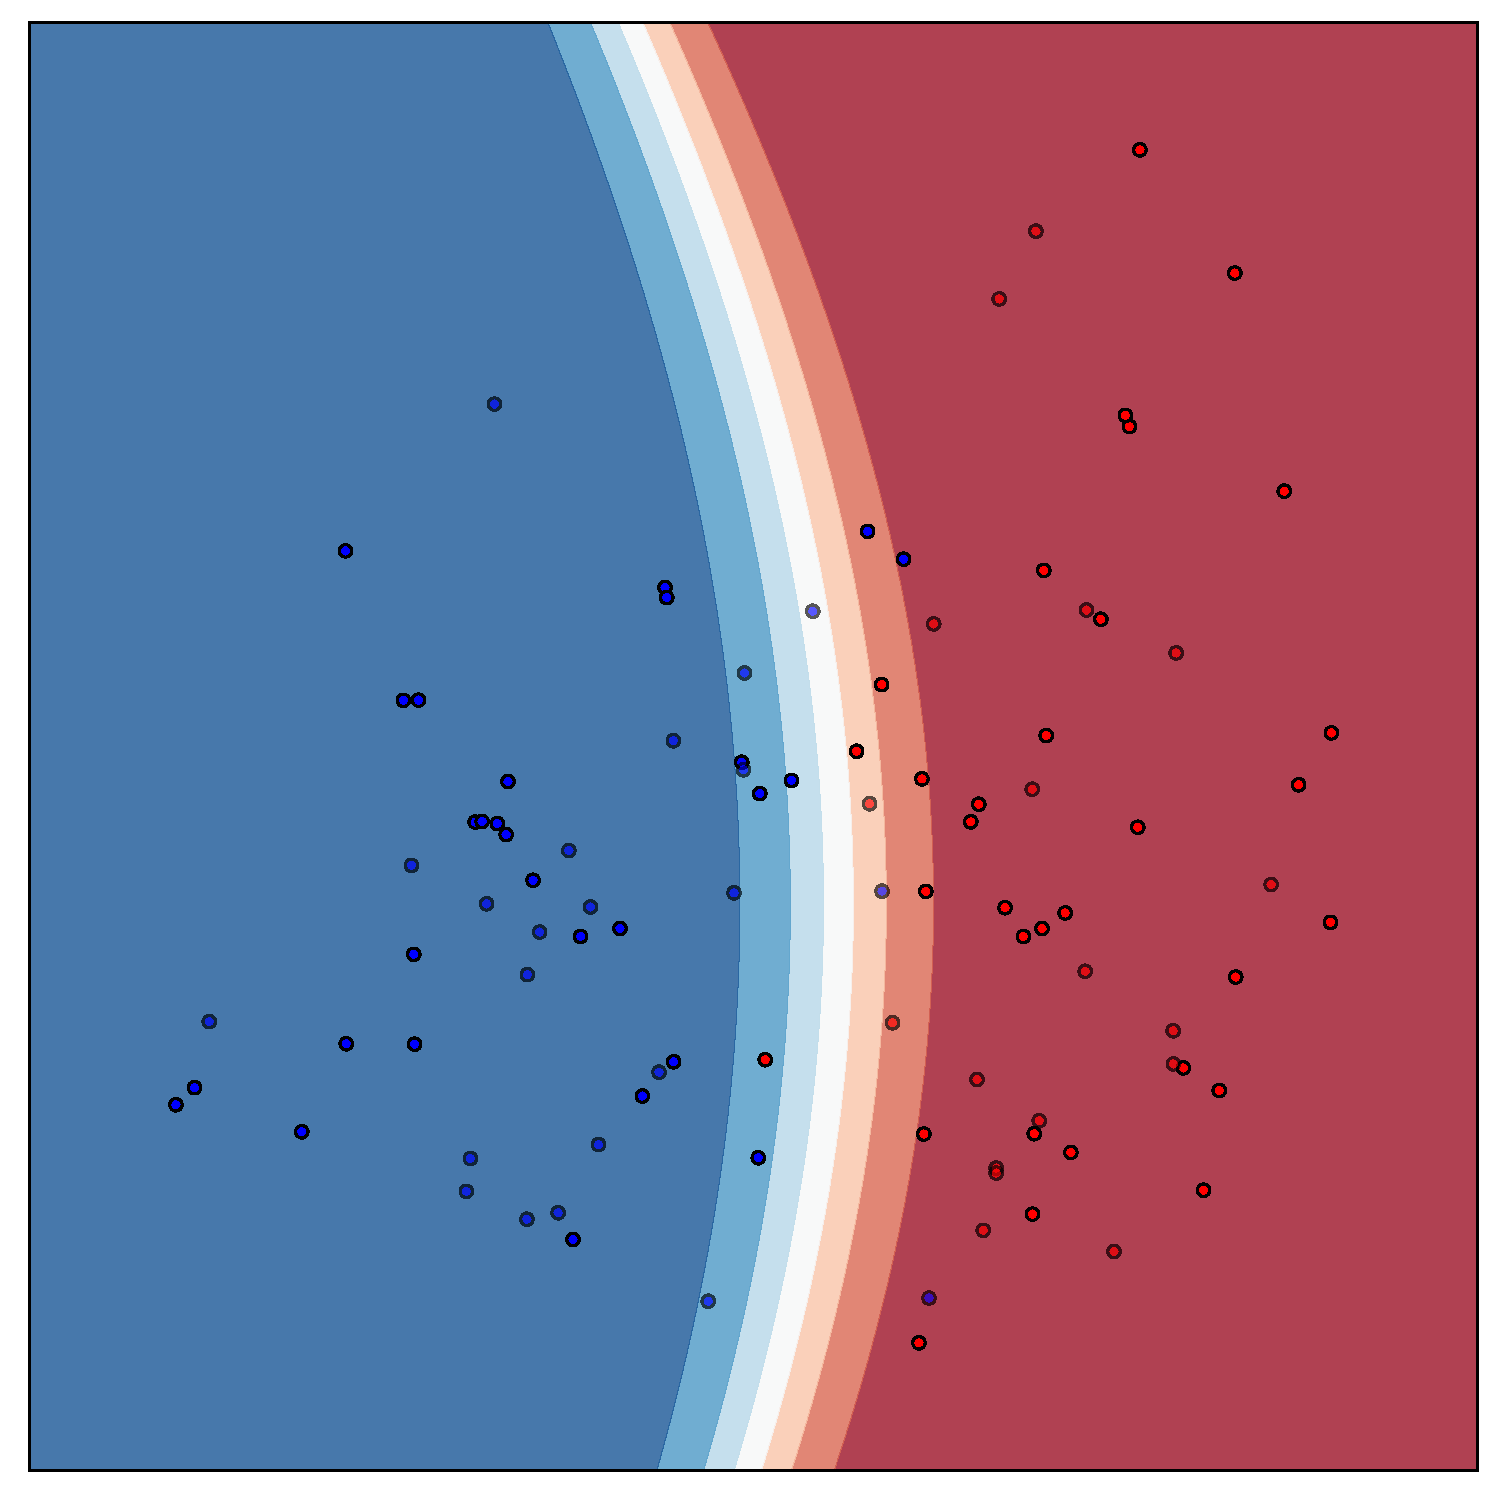
\includegraphics[width=0.75\linewidth]{figures/nb_classification.pdf}
        \label{fig:nb_classification}
    \end{subfigure}
    \caption{
        Illustration of the decision boundary for the logistic regression (left)
        and gaussian naive Bayes (right) for binary classification.
        For logistic regression, the separation is an hyperplane.
        For gaussian naive Bayes, the separation has a dependency on $x \odot x$ and can be non-linear.
        Both bernoulli and multinomial naive Bayes would have a linear separation.
    }
    \label{fig:log_reg_nb_comparison}
\end{figure}

\section{Sparse naive Bayes}\label{sec:snb}

A sparse version of naive Bayes was introduced in 2019~\cite{sparse_naive_bayes}.
They add a sparsity constraint in the Bernoulli and the multinomial optimization problems portrayed above.
It imposes the weight vector $\ww$ to have a number of non-zero entries under a certain threshold $k \in \N$.
That property is similar to the one of the Lasso presented in~\ref{subsubsec:lasso}.
But the sparsity in sparse naive Bayes (SNB) is controlled by an integer $k$ which is
the exact sparsity level desired on the weight vector,
while the Lasso relies on a continuous penalty coefficient $\lambda \in \R$.
This sparsity property makes SNB employable to perform feature selection,
by keeping only the features whose weights are non-zero.
Next sections detail the problem statement, the main results of the authors,
and some applications.

\subsection{Problem statement}\label{subsec:snb_ps}

Let $0 \leq k \leq p$ be a desired level of sparsity.
We wish to train a naive Bayes classifier whose decision boundary depends on at most $k$ features.
For any $\vv \in \R^d$ we note $\norm{\vv}_0$ the number of non-zero entries
(the cardinality) of the vector.
As shown in the previous section~\ref{subsec:nb_bound},
there exist $v \in \R$ and $\ww \in \R^p$ such that the prediction $y(\xx)$ for a new data point $\xx\in\R^p$ is
$\sign(v + \ww^\top\xx)$ for both bernoulli and multinomial naive Bayes.
Furthermore, the $j$th entry of the decision vector $\ww$ is null if and only if $\btheta^-_j = \btheta^+_j$,
where $\btheta^-$ and $\btheta^+$ are the parameters of the loss functions $\lglh_b$ and $\lglh_m$
in~\ref{eq:bernoulli_snb_ll} and~\ref{eq:multinomial_snb_ll} respectively.
Naturally, imposing the constraint $\norm{\btheta^+ - \btheta^-}_0 \leq k$ in the optimization problems
will yield a weight vector $\ww$ with the desired sparsity.
The optimization problems for Bernoulli and multinomial SNB
(shortened BSNB and MSNB respectively) can be phrased as follows:
\begin{equation}\label{eq:bsnb}\tag{BSNB}
    \begin{aligned}
        & \underset{\btheta^+,\, \btheta^-}{\text{maximize}}
        & & \lglh_\text{b}\left( \btheta^+,\, \btheta^- \right)
            \begin{split}
                &&&= \ff_+^\top\log\btheta^+ + (n_+\1 - \ff_+)^\top\log\left( \1 - \btheta^+ \right)\\
                &&&\qquad+ \ff_-^\top\log\btheta^- + (n_-\1 - \ff_-)^\top\log\left( \1 - \btheta^- \right)
            \end{split}\\
        & \text{subject to}
        & & \norm{\btheta^+ - \btheta^-}_0 \leq k.
    \end{aligned}
\end{equation}
\begin{equation}\label{eq:msnb}\tag{MSNB}
    \begin{aligned}
        & \underset{\btheta^+,\, \btheta^-}{\text{maximize}}
        & & \lglh_\text{m}\left( \btheta^+,\, \btheta^- \right) = \ff_+^\top\log\btheta^+ + \ff_-^\top\log\btheta^-\\
        & \text{subject to}
        & & \norm{\btheta^+ - \btheta^-}_0 \leq k\\
        & \text{ and }
        & & \1^\top\btheta^+ = \1^\top\btheta^- = 1.
    \end{aligned}
\end{equation}

\subsection{Main results and resolution}\label{subsec:snb_th}

Surprisingly and despite the combinatorial constraints,
these optimizations problems can be (approximately) solved very efficiently,
with an additional minor cost compared to vanilla naive Bayes.

Especially for the Bernoulli case,
an optimal solution can be computed in closed-form as shown in Theorem~\ref{th:bsnb}.
\begin{theorem}\label{th:bsnb}
    Suppose that $X \in \left\{ 0, 1 \right\}^{n \times p}$ is modeled by the Bernoulli distribution.
    Then, the exact solution to the problem~\ref{eq:bsnb} can be computed.
    First, define $\mt$ and $\uu$ as follows
    \begin{align*}
        \mt &= (\ff^+ + \ff^-) \odot \log\left( \frac{\ff^+ + \ff^-}{n} \right)
                + (n\1 - \ff^+ - \ff^-) \odot \log\left( \1 - \frac{\ff^+ + \ff^-}{n} \right)\\
        \begin{split}
                \uu &= \ff^+ \odot \log \frac{\ff^+}{n^+} + (n^+\1 - \ff^+) \odot \log (\1 - \frac{\ff^+}{n^+})\\
                &\qquad + \ff^- \odot \log \frac{\ff^-}{n^-} + (n^-\1 - \ff^-) \odot \log (\1 - \frac{\ff^-}{n^-})
        \end{split}
    \end{align*}
    Let $\cI$ be the set of $p - k$ smallest elements of $\uu - \mt$, and let
    \begin{equation*}
        {\theta^+_\star}_j = {\theta^-_\star}_j = \frac{1}{n}(f_j^+ + f_j^-)
        \;\forall j \in \cI
        ,\qquad
        {\theta^\pm_\star}_j = \frac{f^\pm_j}{n^\pm}
        \;\forall j \notin \cI
    \end{equation*}
\end{theorem}
Forming the vectors $\ff^-$ and $\ff^+$ is very quick
and takes asymptotically $\cO\left( n \cdot p \right)$ summations.
Then, constructing $\mt$ and $\uu$ can be done in $\cO\left( p \right)$ calculations.
Finding the $k$ largest elements of $\uu - \mt$ takes $\cO\left( p \cdot \log k \right)$ steps.
Finally, constituting $\btheta_\pm^\star$ requires $\cO\left( p \right)$ operations.
In total, the maximizer can be found in $\cO\left( n \cdot p + p \cdot \log k \right)$ steps,
which is very close to the cost $\cO\left( n \cdot p \right)$ of naive Bayes.

In the multinomial case, there is no closed-form solution, but a near-optimal one can be obtained as
stated in Theorem~\ref{th:msnb}.
\begin{theorem}\label{th:msnb}
    Suppose that $X \in \R_+^{n \times p}$ is modeled by the multinomial distribution.
    Then the dual of~\ref{eq:msnb} can be solved very efficiently and a good solution to the primal can be recovered.
    Define $\phi_k : \alpha \mapsto s_k(\hh(\alpha)) + C$ where $C$ is some constant,
    $s_k$ the sum of the k largest values of a vector, and
    \begin{equation*}
        \begin{split}
            \hh(\alpha) &= \ff_+ \odot \log \ff_+ + \ff_- \odot \log \ff_-
                    - (\ff_+ + \ff_-) \odot \log (\ff_+ + \ff_-)\\
                &\qquad - \ff_+ \log \alpha - \ff_- \log (1 - \alpha)
        \end{split}
    \end{equation*}
    $\phi_k$ is the dual of~\ref{eq:msnb} and can be minimized very quickly (with bisection for example)
    as it is a one-dimensional convex convex function.
    Let $\alpha^\star$ be its minimizer, $\cI$ the set of the $p - k$ smallest entries of
    $\hh(\alpha^\star)$, and $B_\pm = \sum_{j \notin \cI} f_i^\pm$.
    A primal point can be reconstructed as follows:
    \begin{equation*}
        {\theta^+_\star}_j = {\theta^-_\star}_j = \frac{f_j^+ + f_j^-}{\1^\top(\ff^+ + \ff^-)}
        \;\forall j \in \cI
        ,\qquad
        {\theta^\pm_\star}_j = \frac{B_+ + B_-}{B_\pm}\frac{f^\pm_j}{\1^\top(\ff^+ + \ff^-)}
        \;\forall j \notin \cI
    \end{equation*}
    Furthermore, it holds that $\psi(k - 4) \leq \phi(k) \leq \psi(k) \leq \phi(k + 4)$,
    implying that the duality gap is small if $\psi(k) - \psi(k - 4)$ is small.
\end{theorem}
Experimentally, the duality gap quickly converges to $0$ as $k$ increases,
and the reconstructed primal point is near-optimal.
The time complexity is once again $\cO(n \cdot p + p \cdot \log k)$,
which is a minor additional cost compared to plain naive Bayes.

The authors experiment SNB on several text datasets,
including AMZN, IMDB, TWTR, MPQA and SST2.
They compare it with more costly methods like the Lasso, $\ell_1$-penalized logistic regression and SVMs.
They obtain competitive test accuracies, while training their models several order of magnitude faster.

\section{Applications}\label{sec:nb_app}

The apparent low complexity of sparse naive Bayes compared to $\ell_1$-penalized methods such as
Lasso, logistic regression or SVMs makes is appealing for very large scale datasets.
We mention here a few applications to which we will come back later\footnote{
    An implementation of sparse naive Bayes can be found~\href{https://github.com/aspremon/NaiveFeatureSelection}{here}.
}.

\subsection{Criteo dataset}\label{subsec:snb_criteo}

As part of a Kaggle competition \emph{Display Advertising Challenge}\footnote{
    The Kaggle competition can be found at
    \href{https://www.kaggle.com/c/criteo-display-ad-challenge}{this address}.
}
in mid-2014, CriteoLabs shared log data collected over one week\footnote{
    The competition's dataset can be downloaded at
    \href{https://labs.criteo.com/2014/02/download-kaggle-display-advertising-challenge-dataset/}{this address}.
}
whose features were undisclosed for confidentiality purposes.
Main characteristics of this dataset can be found in Table~\ref{tab:criteo_dataset}.
\begin{table}[!htb]
    \centering
    \setlength{\tabcolsep}{2pt}
    {\small
    \begin{tabular}{|c|c|c|c|c|}\hline
    \textbf{Samples} & \textbf{Total features} & \textbf{Numerical features} & \textbf{Categorical features} & \textbf{Features after encoding}\\ \hline
    $45\,840\,617$ & $39$  & $13$ & $26$ & $33\,762\,590$ \\ \hline
    \end{tabular}
    }%
    \caption[short]{
        Criteo dataset characteristics.
        Even though the number of features is small,
        most categorical features have millions of categories.
        It makes the training of predicting models particularly challenging as it requires several
        dozens of GB of memory.
    }
    \label{tab:criteo_dataset}
\end{table}
It consists in $\approx 45$ millions of display ads with 39 features,
and a boolean label describing whether or not the ad was clicked by a customer.
Among these 39 features, 26 are categorical and a classical one-hot encoding would end up in millions of features.
This makes the Criteo dataset challenging, as it doesn't fit in the random-access memory after encoding,
and potentially not in the mass storage of a standard computer either.
Even on a small subset of the features, say 10\%,
selecting important features using Lasso or $\ell_1$-penalized logistic regression isn't realistic.
One-hot encoding isn't adapted to that situation.
Another approach would be to one-hot encode for each categorical feature only the most frequent categories,
and put the rest in a category \textit{other}.
The winners of the Kaggle competition used the hashing trick.
It consists in choosing an encoding space size $m$,
for example $m = 2^{20}$,
and defining some hash function $h \colon \text{Categories} \to \left\{ 0, \dots, m - 1 \right\}$.
This approach has several notable advantages.
First, the final encoded feature space $m$ can be adapted depending on the needs and on the computing power.
It may be used in an online fashion without a first pass
(that would be required for one-hot encoding in order to figure out all the existing categories).
Lastly, it naturally handles new labels in the test set that were unseen in the train set
(which would typically need a special \textit{other} category in the one-hot encoding setting).
Collisions between categories are likely to happen,
and even collisions between categories from different features.

We present here in Figure~\ref{fig:criteo_hash_elbow}.
$m = 2^{24} = 16777216$
All the computations are done on a standard workstation (16GB, Intel Core i7 3.60GHz $\times$ 8).
Sparse naive Bayes requires data averages to run,
i.e.\ the sums of the negative and of the positive points.
This part is time consuming but once these sums are computed they can be reused for any sparsity level $k$.
Using a light hash function and PyPy, they were obtained in around 20 minutes.
Only roughly half of the $2^{24}$ hash features were hit by the hash function.
Then, SNB optimum are computed for 1200 log-spaced points using a Python and NumPy implementation of SNB in 1 hour.
In this situation, what makes SNB particularly appealing is the fact that at no moment we need to load the full dataset
in memory.
We are only computing data averages whose shape are much smaller than the full matrix.
Note also that most tasks could even be distributed to speed up the computations.
\begin{figure}
    \centering
    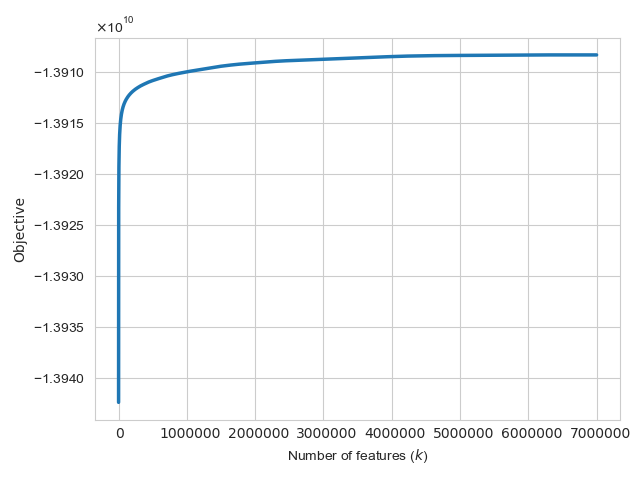
\includegraphics[width=0.75\linewidth, height=0.4\linewidth]{figures/criteo_hash_elbow.png}
    \caption{
        Optimal value of the~\ref{eq:msnb} optimization problem on the Criteo dataset
        as a function of the sparsity parameter $k$.
        Only 1--2 millions of the features explain most of the target vector (elbow heuristic).
    }
    \label{fig:criteo_hash_elbow}
\end{figure}

\bigbreak
Finally, sparse naive Bayes appear as an attractive alternative to the Lasso for the statistics computation
in the knockoff procedure~\ref{subsec:ksc}.


\section{Other fast statistics}\label{sec:other_fast_statistics}

Remember the Lasso Signed Max (LSM) statistics defined in~\ref{eq:lsm}.
\begin{equation}\label{eq:lsm}
    z_j = \sup\{\lambda \mid \hat{\bbeta}_j(\lambda) \neq 0\}
    ,\qquad\quad
    \hat{\bbeta}(\lambda) =
        \underset{\bb}{\argmin}\;
        \frac{1}{2}\big\lVert \yy - \big[ X,\, \tX \big]\bb \big\rVert_2^2 + \lambda\norm{\bb}_1
\end{equation}
The more significant the feature $j$ is,
the higher the first value of $\lambda$ such that it enters the model will be.
That kind of statistics relying on a penalty could be used for other models than the Lasso,
and be potentially easier to compute.
Another possibility is to replace the $\ell_1$ penalty by an $\ell_0$ one.
We find that when this is done for bernoulli and gaussian naive Bayes,
and for centroid classifiers (depicted in Subsection~\ref{subsubsec:centroids}),
the statistics $z_j = \sup\{\lambda \mid \hat{\bbeta}_j(\lambda) \neq 0\}$
can be computed in closed-form.

As a matter of example, for the $\ell_2$ centroids penalized with the $\ell_0$ norm,
the optimization problem is the following one.
\begin{equation}\label{eq:penalized_centroids_averages}
    \hat{\bbeta}(\lambda) = \argmin_{( \btheta^+,\, \btheta^-)}
        \frac{1}{n^+} \sum_{i \in \cI^+} \big\lVert \xx_i - \btheta^+ \big\rVert^2_2
        + \frac{1}{n^-} \sum_{i \in \cI^-} \big\lVert \xx_i - \btheta^- \big\rVert^2_2
        + \lambda \norm{\btheta^+ - \btheta^-}_0
\end{equation}
We find that
\begin{align*}
    z_j = \frac{1}{2}(\bar{\xx}^+_j - \bar{\xx}^-_j)^2
\end{align*}
There is also a very cheap way to compute such values with $\ell_1$ norms in~\ref{eq:penalized_centroids_averages},
with a $\ell_0$ penalization of $\lambda$.

\bigbreak
All these fast heuristics are available in our Python implementation.
In general, they certainly lead to a lower statistical power than more expressive models.
We show experiments with these statistics in Chapter~\ref{ch:exp}.

    \chapter{Efficient knockoffs construction}\label{ch:sdp}

As shown in Chapter~\ref{ch:knockoffs}, in the case of gaussian knockoffs,
$\tX$ can be sampled from a normal distribution $\cN\left( \bupsilon,\, \Upsilon \right)$ whose parameters
$\bupsilon,\, \Upsilon$ are formulated in~\ref{eq:conditional_gaussian_knockoffs2}.
\begin{equation}\label{eq:conditional_gaussian_knockoffs2}
    \tcX \mid \cX \sim \cN\left( \bupsilon, \Upsilon \right)
    ,\qquad\text{where}\quad
    \begin{cases*}
        \bupsilon = \cX - \cX\Sigma^{-1}\diag\{ \bs \}\\
        \Upsilon = \diag\{ \bs \}\left( 2I_{p \times p} - \Sigma^{-1}\diag\{ \bs \} \right)
    \end{cases*}
\end{equation}
More generally, the same parameters are derived by only imposing
$\big[ X; \tX \big]_{\swap\left( S \right)}^\top$ and $\big[ X; \tX \big]^\top$
to have equal first two moments
for any subset
$S \subseteq \left\{ 1, \dots, p \right\}$,
rather than the same distribution.
These formulas are valid for any vector $\bs \in \R^p$ such that $\Omega$
is indeed a covariance matrix (semidefinite positive).
\begin{equation*}
    \Omega = \begin{bmatrix}
        \Sigma & \Sigma - \diag \bs\\
        \Sigma - \diag \bs & \Sigma
    \end{bmatrix}
    \succeq \0_{2p \times 2p}
\end{equation*}
As shown in Proposition~\ref{prop:omega_psd},
this matrix is semidefinite positive if and only if $\0_{p \times p} \preceq \diag \bs \preceq 2 \Sigma$.
The first inequality clearly holds if all the entries of $\bs$ are positive.
It is however trickier to identify all vectors $\bs$ satisfying the second one.

In this chapter, we show why the choice of $\bs$ is important and how to efficiently find an appropriate one
in the high-dimensional setting.
We also form low-rank covariance approximations and procedures to quickly sample $\tcX$.
In the remaining, we note $\Sigma$ the true covariance and $\hat{\Sigma}$ its estimation from the samples $X$
(be it empirical or derived from more sophisticated methods).

\section{Equi-correlated knockoffs}\label{sec:equi}

\subsubsection{A cheap solution}

For any psd matrix $A \in \R^p$, $A + \alpha I_{p \times p}$ has the same eigenvalues as $A$, but shifted by $\alpha$.
It gives a fast and simple way to find a feasible $\bs$:
setting all the entries to the smallest eigenvalue of $\tcove$ (\textit{equi}-correlated knockoffs).
\begin{equation}\label{eq:equi}
    s_j = 2\lambda_{\min}(\cove)
    \quad\text{for all}\quad 0 \leq j \leq p
\end{equation}
The problem of finding the smallest eigenvalue $\lambda_{\min}(\cove)$ can be solved efficiently,
using for instance a singular value decomposition which runs in $\cO(p^3)$ steps~\citep{svd}.

\subsubsection{Why it is not desirable}

For large values of $p$,
the minimum eigenvalue of $\cove$ is likely to be very small,
unless $\cove$ has a substantially special structure.
Let us analyze briefly the covariance of $\big[ \cX; \tcX \big]$
to understand why it is unprofitable for the selection procedure.
If $\tcX$ is built according to~\ref{eq:conditional_gaussian_knockoffs2}, it satisfies
\begin{equation*}
    \begin{cases}
        \cov(\tcX_j,\, \tcX_{j'}) = \cov(\cX_j,\, \cX_{j'}) \text{ for all } j,\,j'\\
        \cov(\cX_j,\, \tcX_{j'}) = \cov(\cX_j,\, \cX_{j'}) \text{ for all } j \neq j'\\
        \cov(\cX_j,\, \tcX_j) = \cov(\cX_j,\, \cX_j) - s_j \text{ for all } j
    \end{cases}
\end{equation*}
First, $\tcX$ has the same internal covariance has $\cX$,
and two distinct original and knockoff features have the same covariance
as the one of the two corresponding original features.
It makes the knockoff features sufficiently close to the original features
to fool the estimator computing the statistics.
However, an original feature $j$ and its corresponding knockoff have a covariance that is smaller the larger $s_j$ is.
If $s_j$ is close to $0$,
$\cX_j$ cannot be distinguished from $\tcX_j$ and the selection is prone to suffer from a low power.
This fact is even more detrimental when $p$ is large as $\lambda_{\min}$ is likely to be very close to $0$.

\section{SDP knockoffs}\label{sec:sdp}

The observation of the previous Section~\ref{sec:equi} motivates us to maximize the entries of $\bs$,
while maintaining the inequality $\diag\bs \preceq \tcovm$.
This can be formulated in the optimization problem~\ref{eq:sdp}.
\begin{equation}\label{eq:sdp}
    \underset{\bs \in \R^p}{\argmax}\;\,
    \sum_{j = 1}^p s_j
    \qquad
    \text{subject to}\quad \begin{cases}
        s_j \geq 0\text{ for all } j\\
        \diag \bs \preceq \tcove
    \end{cases}
\end{equation}
This problem is a structured semidefinite program (SDP) and can be solved efficiently for small values of
$p$ by interior point methods~\citep{sdo_todd, sdp_handbook} for example.
However, it quickly becomes intractable for large values of $p$ (one thousand or more).
In memory, these schemes need to store roughly $\cO(m^2)$ floats
and the time complexity is approximately $\cO\left( m^3 \right)$, where $m$ is the number of constraints
($p$ is this case).
Experimentally, alternating direction~\citep{sdp_admm}
and first order methods like SCS~\citep{sdp_scs} also fail to scale satisfactorily in high dimension.
Figure~\ref{fig:cvx_sdp_times} shows the convergence time of the solvers SCS and MOSEK as a function of $p$.
It makes it clear that different approaches have to be considered when $p$ is more than a few thousands.
Moreover, most solutions returned by these algorithms are actually infeasible because of numerical approximations.
\begin{figure}
    \centering
    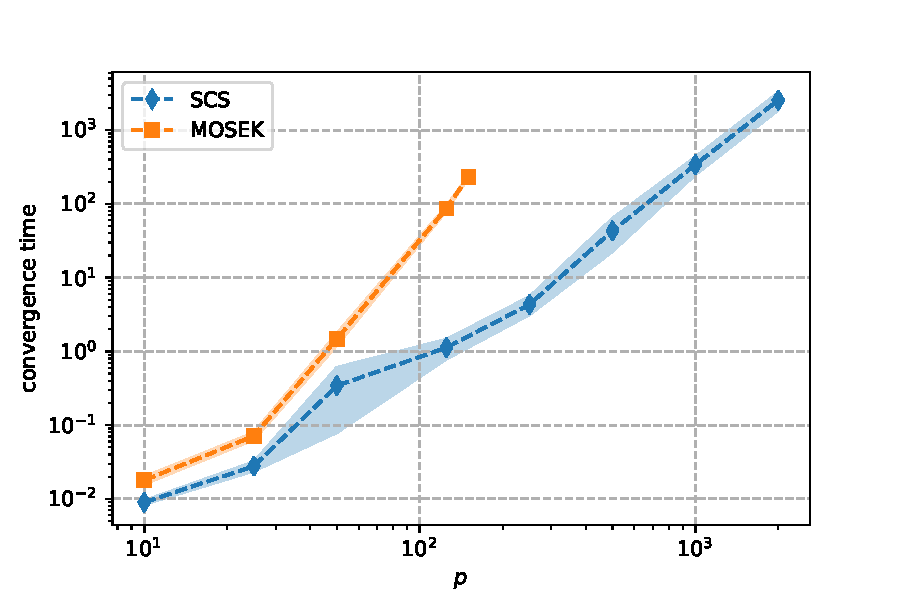
\includegraphics[width=0.8\linewidth, height=0.5\linewidth]{figures/cvx_sdp_times.pdf}
    \caption{
        Time (in seconds) required to converge for SCS (blue) and MOSEK (orange) solvers
        as a function of $p$ in log-log scale.
        Rapidly, MOSEK needs too much memory and can't be run for $p > 150$.
        Both match the theoretical $\cO(p^3)$ rate and SCS already needs 15 minutes for $p = 1000$.
        See Appendix~\ref{sec:cvx_times} for details regarding the random generation of covariance
        matrices $\cove$.
    }
    \label{fig:cvx_sdp_times}
\end{figure}

In order to reduce the computation time~\cite{model_x_knockoffs}
suggest to solve an approximated problem of~\ref{eq:sdp} in 2 steps that we describe below.
\paragraph*{Step 1.}
Pick a block-diagonal approximation $\coveapprox$ of $\cove$ and solve
\begin{equation}\label{eq:sdp_approx}
    \underset{\hat{\bs} \in \R^p}{\argmax}\;\,
    \sum_{j = 1}^p \hat{s}_j
    \qquad
    \text{subject to}\quad \begin{cases}
        \hat{s}_j \geq 0\text{ for all } j\\
        \diag \hat{\bs} \preceq \tcoveapprox
    \end{cases}
\end{equation}
\paragraph*{Step 2.}
Solve the one dimensional maximization
\begin{equation}\label{eq:sdp_approx_1d}
    \underset{\gamma \in \R}{\argmax}\;\,\gamma
    \qquad\text{subject to}\quad
    \diag\left( \gamma \cdot \hat{\bs} \right) \preceq \tcove
\end{equation}
Finally, pick $\bs = \gamma \cdot \hat{\bs}$.
\begin{remark}
    Note that the two extreme options $\coveapprox = I$ and $\coveapprox = \cove$ yield
    the same solutions as solving equi-correlated knockoffs~\ref{eq:equi} and full SDP knockoffs~\ref{eq:sdp} respectively.
\end{remark}
Solving~\ref{eq:sdp_approx_1d} in Step 2 can be done very efficiently using bisection as it is a one-dimensional SDP\@.
The optimization problem~\ref{eq:sdp_approx} is the same as the one in~\ref{eq:sdp},
except for the approximation $\coveapprox$.
To speed up the computations,
$\coveapprox$ can be chosen to be a block-diagonal matrix of $k$ blocks.
The maximization then reduces to $k$ smaller SDPs for which solutions can be found more efficiently.
All the sub-problems being independent, they could even be distributed in several computation nodes.
Picking $\coveapprox$ is a compromise between available computation time and quality of the approximation
(hence ultimate statistical power of the procedure).
The block-diagonal structure can be obtained by reordering columns of $\cove$
with a clustering step grouping similar features (i.e. highly correlated features).

\bigbreak
In practice, the block-diagonal structure is unrealistic.
On top of that, the problem remains intractable when $p$ is a few dozens of thousands,
even if ten groups of features are identified.
The clustering step may also be costly,
and the covariance matrix $\cove$ itself might not even be storable in memory.

\section{A coordinate ascent approach}\label{sec:coordinate_ascent}

We propose here a coordinate ascent algorithm which is proven to converge when coupled with a log-barrier penalty.
It may very well be executed in the block-diagonal arrangement depicted in the previous section.

\subsection{Notations and preliminaries}\label{subsec:notations_preliminaries}

\paragraph{Notations.}
Let $M \in \R^{p \times p}$.
Given two sets of indices $\cI,\,\cJ \in \fset$,
we note $M_{\cI,\,\cJ}$ the $\abs{\cI} \times \abs{\cJ}$ matrix obtained by keeping
the $\abs{\cI}$ rows and $\abs{\cJ}$ columns indexed by $\cI$ and $\cJ$ respectively.
By convenience, an integer $j$ denotes the set $\left\{ j \right\}$ and $j^c$ $\fset \setminus \left\{ j \right\}$
in the matrix subscripting context.
For example, if $M = \begin{bmatrix}
    1 & 2 & 3\\
    4 & 5 & 6\\
    7 & 8 & 9
\end{bmatrix}$,
then $M_{1^c, 1^c} = \begin{bmatrix}
    5 & 6\\
    8 & 9
\end{bmatrix}$
and $M_{1^c, 1} = \begin{bmatrix}
    4\\
    7
\end{bmatrix}$.

\paragraph{Positiveness characterisation.}
Suppose $M$ is structured as
\begin{equation*}
    M = \begin{bmatrix}
        \xi & \yy^\top\\
        \yy & B
    \end{bmatrix}
\end{equation*}
where $B$ is symmetric and invertible.
\begin{lemma}\label{lemma:schur1}
    Using Schur complements (see Appendix~\ref{sec:schur_complement}), it holds that M is psd if and only if
    \begin{equation*}
        B \succeq \0
        \quad\text{and}\quad
        \xi - \yy^\top B^{-1} \yy \geq 0
    \end{equation*}
\end{lemma}
In subscript notations, this is equivalent to $M_{1^c,\, 1^c} \succeq \0$ and
$M_{1,\, 1} - M_{1^c,\, 1}^\top M_{1^c,\, 1^c} M_{1^c,\, 1} \geq 0$.
This statement can be generalized as follows.
For any $j \in \fset$, M is psd if and only if both conditions in~\ref{eq:psd_schur_permutation} are satisfied
\begin{equation}\label{eq:psd_schur_permutation}
    \begin{cases}
        M_{j^c,\, j^c} \succeq \0\\
        M_{j,\, j} - M_{j^c,\, j}^\top M_{j^c,\, j^c} M_{j^c,\, j} \geq 0
    \end{cases}
\end{equation}
\begin{proof}
    Let $j \in \fset$.
    Let $P$ be the permutation matrix swapping columns $1 \leftrightarrow j$ and letting other columns unchanged.
    In two-line form, it is written
    \begin{equation*}
        P = \begin{pmatrix}
                1 & 2 & \dots & j - 1 & j & j + 1 & \dots & p\\
                j & 2 & \dots & j - 1 & 1 & j + 1 & \dots & p
        \end{pmatrix}
    \end{equation*}
    M is psd if and only if $P^\top M P$ is psd.
    $P^\top M P$ is $M$ with lines and columns $1$ and $j$ swapped.
    By applying Lemma~\ref{lemma:schur1} on it, we get the result.
\end{proof}

\subsection{Coordinate ascent}\label{subsec:coordinate_ascent}

Using the characterization~\ref{eq:psd_schur_permutation},
it appears that the feasibility of $\bs$ in SDP~\ref{eq:sdp} is equivalent to the three following conditions,
for any $j \in \fset$
\begin{equation}\label{eq:schur_sdp_constraints}
    \tcove \succeq \diag \bs \succeq \0
    \iff
    \begin{cases}
        \bs \geq \0\\
        \tcove_{j,\, j} - s_j
            - 4\cove_{j^c,\, j}^\top\big( \tcove_{j^c,\, j^c} - \diag \bs_{j^c} \big)^{-1}\cove_{j^c,\, j} \geq 0\\
        \tcove_{j^c,\, j^c} - \diag \bs_{j^c} \succeq \0
    \end{cases}
\end{equation}
This observation motivates the following coordinate approach, as described by~\cite{block_coordinate_sdp}.
Start with a feasible solution $\bs_0$, for example $\bs_0 = \0_p$.
At each iteration, only one coordinate $j$ of $\bs$ will be updated (to optimize a sub-objective),
and the constraints remain satisfied if we pick $s_j$ such that
\begin{equation}\label{eq:sdp_simple_constraints}
    \begin{cases}
        s_j \geq 0\\
        s_j \leq \tcove_{j,\, j}
            - 4\cove_{j^c,\, j}^\top\big( \tcove_{j^c,\, j^c} - \diag \bs_{j^c} \big)^{-1}\cove_{j^c,\, j}
    \end{cases}
\end{equation}
Consequently, we set $s_j$ to the maximum value keeping the constraints valid,
that is
\begin{equation*}
s_j = \max\Big( \tcove_{j,\, j}
    - 4\cove_{j^c,\, j}^\top\big( \tcove_{j^c,\, j^c} - \diag \bs_{j^c} \big)^{-1}\cove_{j^c,\, j}
    ,\, 0 \Big)
\end{equation*}
Unfortunately, this method is not guaranteed to converge to the global maximum, even when the problem is concave.
A slight modification depicted in the next section will correct that.

\subsection{Log-barrier}\label{subsec:log_barrier}

Instead of optimizing~\ref{eq:sdp},
we absorb the constraint $\tcove \succeq \bs$ into the objective by penalizing solutions
too close to the feasibility frontier, as described by~\citet[§11.3]{convex_optimization}.
It depends on the additional term
$\lambda \cdot \log\det\big( \tcove - \diag\bs \big)$
for some coefficient $\lambda > 0$:
\begin{equation}\label{eq:sdp_log_barrier}
    \underset{\bs \in \R^p}{\argmax}\;\,
    \sum_{j = 1}^p s_j
    + \lambda \cdot \log\det\big( \tcove - \diag\bs \big)
    \qquad
    \text{subject to}\quad
    s_j \geq 0\text{ for all } j
\end{equation}
where we consider that $\log 0 = -\infty$.
Intuitively, a solution $\bs$ such that the minimum eigenvalue of $\tcove - \diag\bs$ gets too close to $0$
will be penalized by this $\log$ term.

\bigbreak
The following lemma will be helpful to compute the determinant.
\begin{lemma}
    If $M = \begin{bmatrix}
        \xi & \yy^\top\\
        \yy & B
    \end{bmatrix}$,
    then
    \begin{align*}
        \det\left( M \right) &= \det\big( \xi - \yy^\top B^{-1} \yy \big) \cdot \det\left( B \right)\\
        &= \big( \xi - \yy^\top B^{-1} \yy \big) \cdot \det\left( B \right)
    \end{align*}
\end{lemma}
\begin{proof}
    It is an immediate consequence of the formula giving the determinant of a block matrix
    reported in Appendix~\ref{sec:block_matrix_det}.
\end{proof}
With subscript notations, this identity can be noted as
$\det\left( M \right) = \big( M_{1,\, 1} - M_{1^c,\, 1}^\top M_{1^c,\, 1^c}^{-1} M_{1^c,\, 1} \big)
    \cdot\det\left( M_{1^c,\, 1^c} \right)$.
Employing the same idea as in~\ref{eq:psd_schur_permutation},
it can further be generalized to
\begin{equation*}
    \det\left( M \right) = \big( M_{j,\, j} - M_{j^c,\, j}^\top M_{j^c,\, j^c}^{-1} M_{j^c,\, j} \big)
        \cdot\det\left( M_{j^c,\, j^c} \right)
\end{equation*}
for any $j \in \fset$.
By applying this to $\log\det\big( \tcove - \diag\bs \big)$,
we get that for any $j$,
\begin{equation*}
    \log\det\big( \tcove - \diag\bs \big) =
        \log\big( \tcove_{j,\, j} - s_j - 4\cove_{j^c,\, j}^\top Q_j^{-1} \cove_{j^c,\, j} \big)
            + \log\det\left( Q_j \right)
\end{equation*}
where $Q_j = \tcove_{j^c,\, j^c} - \diag\bs_{j^c}$ does not depend on $s_j$.

\bigbreak
Again, we start from a feasible solution $\bs^{(0)} = \0_p$ and perform coordinate ascent.
At each iteration, a new coordinate $j$ is updated
and we take advantage of the fact that $Q_j$ doesn't depend on $s_j$.
The function
\begin{equation*}
    \alpha \mapsto \alpha
        + \lambda\log\big( \tcove_{j,\, j} - \alpha - 4\cove_{j^c,\, j}^\top Q_j^{-1} \cove_{j^c,\, j} \big)
\end{equation*}
is concave and setting its derivative to $0$ yields that its maximum is
\begin{equation*}
    \alpha^\star = \tcove_{j,\, j} - 4\cove_{j^c,\, j}^\top Q_j^{-1} \cove_{j^c,\, j} - \lambda
\end{equation*}
The $j$th coordinate is therefore updated as $s_j \leftarrow \max\left( \alpha^\star,\, 0 \right)$.
Note in particular that this update maintains the feasibility
conditions~\ref{eq:sdp_simple_constraints} for any value of $\lambda$.

\citet[§11.3]{convex_optimization} suggest that picking $\lambda = \epsilon / p$ will yield an
$\epsilon$-optimal solution.
In practice, an initial $\lambda_0$ is picked and it is multiplied by a decay rate
$0 < \mu < 1$ after each coordinate cycle to refine the solution.
This scheme can be proven to converge to the maximum
of the modified objective~\ref{eq:sdp_log_barrier}.
It is indeed a particular case of ~\citet[Theorem~3]{block_coordinate_sdp},
which applies in this case as the constraints are simple,
i.e. $\bs \geq \0$ is of the form $L \leq \diag\bs \leq U$.

\bigbreak
This log-barrier algorithm is summarized in pseudo-code in Algorithm~\ref{alg:coordinate_ascent_log_barrier}.
The bottleneck is the inversion of the matrix
$Q_j \in \R^{(p - 1) \times (p - 1)}$ in line~\ref{alg:line:q_inv} which takes $\cO\left( p^3 \right)$ steps.
As it is done in every inner iteration, the time complexity of Algorithm~\ref{alg:coordinate_ascent_log_barrier} is
$\cO\left( n_\text{iters} \cdot p^4 \right)$ when implemented naively.
It is possible to design a version running in $\cO\left( n_\text{iters} \cdot p^3 \right)$ steps instead.
To see this, note $A = \tcove - \diag\bs \in \R^{p \times p}$.
At each iteration $j$, $Q_j$ is a principal sub-matrix of $A$ and its inverse can efficiently be computed
(in $\cO\left( p^2 \right)$ steps) from the one of $A$~\citep{submatrix_inverse}.
On top of that, when a coordinate $s_j$ changes,
$A$ is only modified with a rank-$1$ update.
Its new inverse can efficiently be computed ($\cO\left( p^2 \right)$ steps)
using for example Sherman-Morrison formula
(see Appendix~\ref{ch:linear_algebra})
or Cholesky rank-$1$ updates~\citep{cholesky_rank_1} which are more stable numerically.
In Appendix~\ref{ch:cython_acceleration} we give a Cython implementation example.
\begin{algorithm}[t]
    \caption{Coordinate ascent with log-barrier}\label{alg:coordinate_ascent_log_barrier}
    \begin{algorithmic}[1]
        \State \textbf{Input:} $\cove$, barrier coefficient $\lambda$, decay $\mu$, $\bs^{(0)} = \0_p$
        \State $\bs = \bs^{(0)}$
        \Repeat
        \For{$j = 1,\,\dots,\, p$}
        \State $Q_j = \tcove_{j^c,\, j^c} - \diag\bs_{j^c}$
        \State $s_j = \max\big( \tcove_{j,\, j} - 4\cove_{j^c,\, j}^\top Q_j^{-1} \cove_{j^c,\, j} - \lambda,\, 0 \big)$\label{alg:line:q_inv}
        \EndFor
        \State $\lambda = \mu \cdot \lambda$
        \Until{stopping criteria}
    \end{algorithmic}
\end{algorithm}

\section{Low-rank covariance approximation}\label{sec:low_rank_sigma}

Covariance estimation in the high-dimensional setting ($p > n$ where $n$ is the number of samples)
is challenging as the sample (empirical) covariance is not accurate.
On top of that,
if $p$ is larger than $20\,000$ it becomes challenging to solely store the full matrix in the memory
of a standard computer.
Hopefully, big data matrices and especially correlation matrices often have an underlying low-rank structure,
or at least can be approximated adequately by such a low-rank estimate~\citep{big_data_low_rank}.
An intuitive explanation is that only a small number of latent features explain most of the data.

\subsection{Factor model}\label{subsec:factor_model}

We approximate the covariance $\cove$ with the following structure
\begin{equation}\label{eq:low_rank_structure}
    \cove = D + U \Lambda U^\top
\end{equation}
where $U \in \R^{p \times k}$ has orthogonal columns ($U^\top U = I_k$),
and both $D \in \R^{p \times p},\, \Lambda \in \R^{k \times k}$
are diagonal and psd.
$k$ is typically much lower than $p$ to save has much memory and computations as possible.

In the case where $X$ is reasonably large,
the decomposition~\ref{eq:low_rank_structure} for the empirical covariance can be obtained as follows.
First factorize $X = P \Delta Q^T$ with SVD~\citep{svd}.
Then (assuming columns are centered),
\begin{align*}
    \cove &= \frac{1}{n}X^\top X\\
    &= \frac{1}{n}Q \Delta^2 Q^\top
\end{align*}
From this, building a rank-$k$ approximation of $\cove$ is easily done by keeping its top $k$ eigenvalues,
that is
\begin{equation*}
    \Lambda = \Delta^2_{:k,\, :k} \qquad\qquad U = Q_{:,\, :k}
\end{equation*}
Then set $D = \diag^2\max \big( \cove - U \Lambda U^\top,\, \0_{p \times p} \big)$
to be the diagonal psd matrix containing
the difference between $\cove$ and the low-rank approximation.
None of these steps requires to form the full covariance matrix $\cove$, which might not fit in memory.

As pointed out earlier, the empirical covariance estimator performs poorly in high dimension.
Shrunk estimators like the one proposed by~\cite{ledoit_wolf} are proven to be often superior in that situation.
Suppose again that $\cove = \frac{1}{n}X^\top X$ is the empirical estimator.
Note $\mu = \Tr( \cove ) / p$ and $\delta$ a shrinkage coefficient.
The shrunk covariance estimator is then given by
\begin{equation*}
    \cove_\delta = (1 - \delta)\cove + \delta\mu I
\end{equation*}
The same decomposition strategy can be employed,
but this time $\cove_\delta = Q\big[ (1 - \delta) \Delta^2 / n + \delta\mu I \big] Q^\top$.
Finding the optimal coefficient $\delta$ can be done in $\cO\left( n \cdot p \right)$ steps
and without extra memory, provided that we know the decomposition of $X$.

Randomized SVD algorithms~\citep{random_svd} may be employed
in the case where computing the exact SVD decomposition of $X$ is too costly,
when $X$ doesn't even fit in memory,
or simply to speed-up the factorization process.
Without the full SVD, computing the optimal shrinkage coefficient $\delta$ is more costly
but can be done in $\cO\left( n^2 \cdot p \right)$ steps and without extra memory.
Rather than simply computing a low-rank approximation $U \Lambda U^\top$ and then $D$,
these randomized estimations allow to achieve alternating descent on $U$ and $D$ without constructing $\cove$.
Nonetheless, one single step seems to be often very close to a local minimum.
We implement such algorithms and find that they scale moderately well with $n$ and $p$.

\bigbreak
In the following sections,
we suppose that the decomposition $\cove = D + U \Lambda U^\top$
was computed.
Even in the (likely) case where the covariance matrix is not exactly diagonal plus low-rank,
this approximating structure is general enough to yield satisfying results.

\subsection{Low-rank coordinate ascent}\label{subsec:low_rank_sdp}

The complexity of Algorithm~\ref{alg:coordinate_ascent_log_barrier} can be drastically reduced
to $\cO\left( n_\text{iters} \cdot p \cdot k^2 \right)$
by taking advantage of the special structure of $\cove$.
Remember that at each iteration $j$,
only the coordinate $j$ of $\bs$ is updated
\begin{equation*}
    s_j \leftarrow \max(\alpha^\star,\, 0)
    \quad\text{with}\quad
    \alpha^\star = \tcove_{j,\, j} - 4\cove_{j^c,\, j}^\top Q_j^{-1} \cove_{j^c,\, j} - \lambda
\end{equation*}
where $Q_j = \tcove_{j^c,\, j^c} - \diag\bs_{j^c}$.
Note $V = U \sqrt{\Lambda}$ so that $\cove = D + VV^\top$.
Then we get that
\begin{equation*}
    Q_j = 2D_{j^c,\, j^c} - \diag\bs_{j^c} + 2V_{j^c,\, :}V_{j^c,\, :}^\top
\end{equation*}
where the subscript `:` denotes that all columns (or rows) are kept.
By writing $F_j = 2D_{j^c,\, j^c} - \diag\bs_{j^c}$ and $A_j = V_{j^c,\, :}^\top F_j^{-1} V_{j^c,\, :}$,
the Woodbury formula (see Appendix~\ref{sec:sherman}) gives that
\begin{align*}
    Q_j^{-1} &=
        F_j^{-1} - 2F_j^{-1}V_{j^c,\, :}
            \big( I_k + 2V_{j^c,\, :}^\top F_j^{-1} V_{j^c,\, :} \big)^{-1}
                V_{j^c,\, :}^\top F_j^{-1}\\
    &= F_j^{-1} - 2F_j^{-1}V_{j^c,\, :}
        \big( I_k + 2A_j \big)^{-1}
            V_{j^c,\, :}^\top F_j^{-1}
\end{align*}
Using this, the inner-loop update $\alpha^\star$ can be written as
\begin{align}\label{eq:low_rank_alpha}
    \alpha^\star &=
        \tcove_{j,\, j}
        - 4\cove_{j^c,\, j}^\top F_j^{-1} \cove_{j^c,\, j}
        - \lambda
        + 8\cove_{j^c,\, j}^\top F_j^{-1} V_{j^c,\, :}
        \big( I_k + 2A_j \big)^{-1}
        V_{j^c,\, :}^\top F_j^{-1}\cove_{j^c,\, j}\nonumber\\[5pt]
    &= \underbrace{
        \tcove_{j,\, j}
        - 4V_{j,\, :} A_j V_{j,\, :}^\top
        - \lambda
    }_\text{$(*)$}
    + \underbrace{8V_{j,\, :} A_j
        \big( I_k + 2A_j \big)^{-1}
        A_j V_{j,\, :}^\top
    }_\text{$(**)$}
\end{align}
where we used the fact that
$\cove_{j^c,\, j} = D_{j^c,\, j} + V_{j^c,\, :}V_{j,\, :}^\top = V_{j^c,\, :}V_{j,\, :}^\top$.

Forming the matrix $A_j$ at each iteration would be very costly.
But if we note $F = 2D - \diag\bs$ and $A = V^\top F^{-1} V$,
it appears that $A_j$ is a rank-1 update of $A$
\begin{align*}
    A_j &= V_{j^c,\, :}^\top F_j^{-1} V_{j^c,\, :}\\
    &= A - F_{j,\, j} \cdot V_{j,\, :}^\top V_{j,\, :}
\end{align*}
Therefore, we can simply build $A$ at the beginning and update it efficiently to make $A_j$.
Using this, the term $(*)$ in~\ref{eq:low_rank_alpha} can be easily evaluated in $\cO\left( k^2 \right)$ steps.
The term $(**)$ involves the computation of the inverse of $B_j = I_k + 2A_j$.
But again, $B_j$ is a rank-1 update of $B = I_k + 2A$,
which can be computed once
and updated with Sherman-Morrison (Appendix~\ref{ch:linear_algebra})
or Cholesky rank-$1$ updates~\citep{cholesky_rank_1}.
Finally, when $s_j$ is updated, the coordinate $(j,\, j)$ of $F$ is changed,
which induces a rank-1 update of $A$.
All these operations can be done in $\cO\left( k^2 \right)$ steps.
The matrix $F$ being diagonal,
it requires only $p$ floats to be stored and its inversion is trivial.

\begin{algorithm}
    \caption{Low-rank coordinate ascent}\label{alg:low_rank_coordinate_ascent}
    \begin{algorithmic}[1]
        \State \textbf{Input:} approximation $\cove = D + U \Lambda U^\top$, barrier coefficient $\lambda$,
            decay $\mu$, $\bs^{(0)} = \0_p$
        \State $\bs = \bs^{(0)}$
        \State $V = U \sqrt{\Lambda}$
        \Repeat
        \For{$j = 1,\,\dots,\, p$}
        \State $F_j = 2D_{j^c,\, j^c} - \diag\bs_{j^c}$
        \State $A_j = V_{j^c,\, :}^\top F_j^{-1} V_{j^c,\, :}$
        \State $\alpha^\star = \tcove_{j,\, j} - 4V_{j,\, :}^\top A_j V_{j,\, :} - \lambda + 8V_{j,\, :}^\top A_j \big( I_k + 2A_j \big)^{-1} A_j V_{j,\, :}$
        \State $s_j = \max\left( \alpha^\star,\, 0 \right)$
        \EndFor
        \State $\lambda = \mu \cdot \lambda$
        \Until{stopping criteria}
    \end{algorithmic}
\end{algorithm}
\begin{figure}
    \centering
    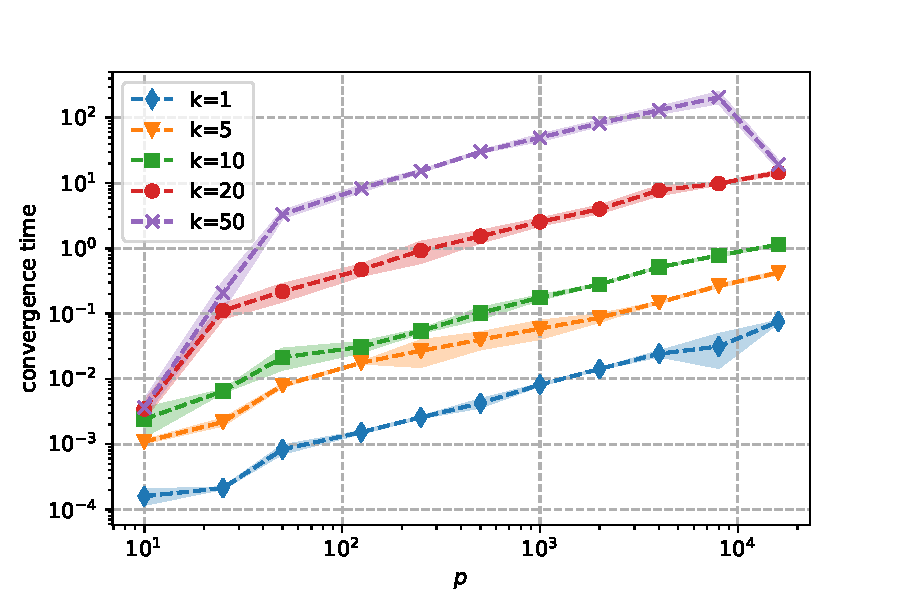
\includegraphics[width=0.8\linewidth, height=0.5\linewidth]{figures/low_rank_times.pdf}
    \caption{
        Convergence times of the low-rank coordinate ascent algorithm~\ref{alg:low_rank_coordinate_ascent}
        as a function of $p$ and $k$.
        It confirms the theoretical $\cO(n_{\text{iters}} \cdot p \cdot k^3)$ rate.
        In practice,
        the algorithm converges much faster to an appropriate solution when using a larger tolerance threshold.
        See Appendix~\ref{sec:coordinate_ascent_data} for details regarding the random data generation.
    }
    \label{fig:low_rank_times}
\end{figure}

This scheme is summarized in Algorithm~\ref{alg:low_rank_coordinate_ascent}.
It uses at most $\cO\left( p \cdot k \right)$ memory
and the time complexity is $\cO\left( n_\text{iters} \cdot p \cdot k^2 \right)$, as stated above.
We make a Cython implementation which is available in the released Python package.
Because of numerical instabilities, we completed experiments with a version inverting the matrix
$I_k + 2A_j$ at each iteration, leading to a higher time complexity of
$\cO\left( n_\text{iters} \cdot p \cdot k^3 \right)$.
Figure~\ref{fig:low_rank_times} shows the convergence times obtained in these experiments,
as a function of $p$ and $k$.
It demonstrates that the scalability is much better than with SCS,
thanks to the low-rank approximation and the fact that coordinate ascent
is particularly well-suited to this optimization problem.
Even with $100\,000$ features, the convergence could be obtained in a few minutes.
We hope to prevent numerical instabilities in future versions and attain the
$\cO\left( n_\text{iters} \cdot p \cdot k^2 \right)$ time complexity.

\subsection{Efficient low-rank sampling}\label{subsec:low_rank_sampling}

In this section, we detail briefly how to sample knockoffs $\tcX$ once
a feasible solution $\bs$ is computed,
and in the special case where $\cove = D + U\Lambda U^\top$.
As shown in Section~\ref{subsec:gaussian_knockoffs},
$\tcX$ is sampled from the following conditional distribution
\begin{equation}\label{eq:conditional_gaussian_knockoffs3}
    \tcX \mid \cX \sim \cN\left( \bupsilon, \Upsilon \right)
    ,\qquad\text{where}\quad
    \begin{cases*}
        \bupsilon = \cX - \cX\Sigma^{-1}\diag\{ \bs \}\\
        \Upsilon = \diag\{ \bs \}\left( 2I_{p \times p} - \Sigma^{-1}\diag\{ \bs \} \right)
    \end{cases*}
\end{equation}
A classical approach to sample
$\zz \sim \cN\left( \bupsilon,\, \Upsilon \right)$
from a multivariate normal distribution is to sample first a vector
$\tilde{\zz} \in \R^p$ from $\cN\left( 0,\, 1 \right)$,
and then pose $\zz = \bupsilon + L\tilde{\zz}$,
where $L$ is a lower Cholesky factorization of $\Upsilon$.
This uses the fact that if $\xx \sim \cN\big( \mu,\, \Sigma \big)$,
then
\begin{equation}\label{eq:affine_transformation}
    A\xx + \bb \sim \cN\big( A\bmu + \bb,\, A\Sigma A^\top \big)
\end{equation}
Note that this scheme works even if $L$ is not lower-triangular,
but simply satisfies $LL^\top = \Upsilon$.

\bigbreak
As $\Upsilon$ is a $p \times p$ matrix we may not want to store it in memory,
nor compute a Cholesky factorization (which takes $\cO\left( p^3 \right)$ steps).
We show here how to factorize $\Upsilon$ in a cheap way,
requiring only $\cO\left( k \cdot p \right)$ memory and $\cO\left( k\cdot p^2 \right)$ operations.
We note $S = \diag\bs$, so that$\Upsilon = 2S - S\cove^{-1}S$.
Using the low-rank structure $\cove = D + U\Lambda U^\top$,
the Woodbury formula (see Appendix~\ref{sec:sherman}) gives
\begin{align*}
    \cove^{-1} &= (D + UU^\top)^{-1}\\
    &= D^{-1} - D^{-1}U(I_k + U^\top D^{-1}U)^{-1}U^\top D^{-1}
\end{align*}
Note $L \in \R^{k \times k}$ the lower Cholesky factorization of
$(I_k + U^\top D^{-1}U)^{-1}$ (which can be computed efficiently if $k$ is small),
$V = SD^{-1}UL \in \R^{p \times k}$,
and $C = 2S - SD^{-1}S$.
Then the covariance reduces to
\begin{equation*}
    \Upsilon = C + VV^\top
\end{equation*}
where $C$ is diagonal and $VV^\top$ has rank at most $k$.
$C$ is not necessarily psd, which will force us to sample from a complex normal distribution.
Let $H$ be a complex square-root of $C$ (thus, potentially with imaginary numbers on the diagonal),
and $P = H^{-1}V \in \R^{p \times k}$.
Then,
\begin{equation*}
    \Upsilon = H \left( I_{p \times p} + PP^\top \right) H^\top
\end{equation*}
$\left( I_{p \times p} + PP^\top \right)$ can be factorized in the following way.
Note
\begin{equation*}
    W = \left(I_{k \times k} + \sqrt{I_{k \times k} + P^\top P}\right)^{-1} \in \R^{k \times k}
\end{equation*}
where the square-root is a $k \times k$ matrix root (which can again be computed efficiently if $k$ is small).
Then
\begin{equation*}
    I_{p \times p} + PP^\top = BB^\top
    ,\qquad
    \text{where}
    \quad
    B = I_{p \times p} + PWP^\top
\end{equation*}
Finally, we note $M = HB$ and we have that $\Upsilon = MM^\top$.
$B$ is $p \times p$ but we never have to fully evaluate it;
instead only $W$ and $P$ can be stored and matrix multiplications are then at most $p \times k$.

$M$ is a complex matrix so we cannot directly use the property~\ref{eq:affine_transformation}.
But if $\cX \sim \cN(\0,\, I)$ and $\cY = i\cX$,
then $\operatorname{Im}\left( M\cY \right) \sim \cN(\0,\, MM^\top = \Upsilon)$.
Using this scheme, we can draw dozens of thousands knockoff samples in a few seconds without explicitely
building $\cove$ nor $\Upsilon$.

    \chapter{Experiments}\label{ch:exp}

In this chapter,
we show experiments performed on genetic data.
That kind of data is usually high dimensional.
For this reason, the tools developed in the previous chapters are particularly suited to solve it.

\section{Setup}\label{sec:exp_setup}

\subsection{Genetic data}\label{subsec:genetic_data}

\footnote{
    Data available at \href{https://amp.pharm.mssm.edu/archs4/download.html}{this address},
    under the filename \texttt{human\_matrix.h5 v8}.
}

\begin{table}[!htb]
    \centering
    \setlength{\tabcolsep}{2pt}
    {\small
        \begin{tabular}{|c|c|c|}\hline
        \textbf{Samples} & \textbf{Total features} & \textbf{N}\\ \hline
        $42000$ & $350000$  & $13$\\ \hline
        \end{tabular}
    }%
    \caption[short]{
        ARCHS4 dataset
    }
    \label{tab:archs4_dataset}
\end{table}

\section{Results}\label{sec:exp_results}

    \cleardoublepage
\chapter*{Conclusion}
\markboth{Conclusion}{Conclusion}
\addcontentsline{toc}{chapter}{Conclusion}

In this master thesis,
we investigated high-dimensional feature selection
in the gaussian knockoffs framework setting.
In high dimension, nearly all the steps of the selection procedure become challenging,
and in particular the construction of the knockoff features,
and the computation of statistics associated to each aggregated feature.

Building knockoffs inducing a high statistical power relies on the optimization of a semidefinite program.
Hopefully, the structure and the simple bounds of this SDP


    %%%%%%%%%%%%%%%%%%%%%%%%%%%%%%%%%%%%%%%%%%%%%%
    %%%%% TAIL: Bibliography, Appendix, CV
    %%%%%%%%%%%%%%%%%%%%%%%%%%%%%%%%%%%%%%%%%%%%%%
    \appendix
\chapter{Data generation details}\label{ch:appendix_data}

\section{SCS and MOSEK convergence times}\label{sec:cvx_times}

Experiments were run in Python using CVX~\cite{cvx} through the Python wrapper CVXPY~\cite{cvxpy}.
Table~\ref{tab:cvx_times_ps} shows the values of $p$ that were used.
We restrained the parameter $p$ for MOSEK as it didn't scale as well as SCS\@.
\begin{table}[!htb]
    \centering
    \setlength{\tabcolsep}{2pt}
    {\small
    \begin{tabular}{|c|c|}\hline
    \textbf{SCS} & \textbf{MOSEK}\\ \hline
        10 & 10\\ \hline
        25 & 25\\ \hline
        50 & 50\\ \hline
        125 & 125\\ \hline
        250 & 150\\ \hline
        500 &\\ \hline
        1000 &\\ \hline
        2000 &\\ \hline
    \end{tabular}
    }%
    \caption[short]{
        Orders of matrices used.
    }
    \label{tab:cvx_times_ps}
\end{table}
For each $p$, 5 replications were performed with matrices of the form $M = D + U \Lambda U^\top$ where $D$ is diagonal,
$\diag D \sim \cU\left[ 0,\, 1 \right]$, $U \in \R^{p \times k}$ for $k = 1,\, 5,\, 10,\, 20,\, 50$
are orthonormal random matrices, and $\Lambda \in \R^{k \times k}$ is diagonal and
$\diag \Lambda^2 \sim \cU\left[ 0,\, 1 \right]$.
No significant difference was measured when changing $k$, even for large values.
The convergence is however much slower if $D$ is scaled up.

\section{Coordinate ascent}\label{sec:coordinate_ascent_data}

\chapter{Linear algebra notes}\label{ch:linear_algebra}

In this section, we state and prove some useful linear algebra facts.

\section{Schur complement and positive definiteness}\label{sec:schur_complement}

Let $X = \begin{bmatrix}
             A & B^\top\\
             B & C
    \end{bmatrix}$
be a symmetric matrix where $A$ and $C$ are invertible.
\begin{definition}
    The Schur complements $X_{/A}$ and $X_{/C}$ are defined as follows:
    \begin{equation*}
        X_{/A} = C - B A^{-1} B^\top
        ,\qquad
        X_{/C} = A - B^\top C^{-1} B
    \end{equation*}
\end{definition}
Schur complements give a way to characterize the fact that X is positive definite and positive semidefinite.
\begin{lemma}
    The following three properties are equivalent:
    \begin{enumerate}
        \item $X \succ \0$
        \item $A \succ \0$ and $X_{/A} \succ \0$
        \item $C \succ \0$ and $X_{/C} \succ \0$
    \end{enumerate}
    As well as the three following:
    \begin{enumerate}
        \item $X \succeq \0$
        \item $A \succ \0$ and $X_{/A} \succeq \0$
        \item $C \succ \0$ and $X_{/C} \succeq \0$
    \end{enumerate}
\end{lemma}
\begin{proof}
    $X$ can be factorized as follows
    \begin{equation*}
        X = \begin{bmatrix}
            I & \0\\
            B^\top C^{-1} & I
        \end{bmatrix}^\top
        \begin{bmatrix}
            A - B^\top C^{-1}B & \0\\
            \0 & C
        \end{bmatrix}
        \begin{bmatrix}
            I & \0\\
            B^\top C^{-1} & I
        \end{bmatrix}
    \end{equation*}
    which means that $X = Q^\top D Q$ where $D$ is a block-diagonal matrix.
    Therefore $X \succ \0$ (resp. $\succeq \0$) if and only if $D \succ \0$ (resp. $\succeq \0$),
    which is equivalent to its diagonal blocks to be $\succ \0$ (resp. $\succeq \0$).
    To get the same result with the complement $X_{/A} = C - B A^{-1} B^\top$,
    we use the factorization
    \begin{equation*}
        X = \begin{bmatrix}
            I & \0\\
            BA^{-1} & I
        \end{bmatrix}
        \begin{bmatrix}
            A & \0\\
            \0 & C - BA^{-1}B^\top
        \end{bmatrix}
        \begin{bmatrix}
            I & \0\\
            BA^{-1} & I
        \end{bmatrix}^\top
    \end{equation*}
\end{proof}

Consider the particular partition
$X = \begin{bmatrix}
    \xi & \yy^\top\\
    \yy & B
\end{bmatrix}$
where $B$ is invertible.
Then a direct application of the theorem above gives that
\begin{equation*}
    \begin{cases}
        X \succ \0 \iff B \succ \0 \text{ and } \xi > \yy^\top B^{-1} \yy\\
        X \succeq \0 \iff B \succ \0 \text{ and } \xi \geq \yy^\top B^{-1} \yy
    \end{cases}
\end{equation*}

More results regarding Schur complements can be found in~\cite{schur_complement}.
A generalization involving pseudo-inverses of $A$ and $C$ when they are singular is possible.

\section{Sherman–Morrison–Woodbury formula}\label{sec:sherman}

The Sherman-Morrison formula gives a way to calculate the inverse of the sum of an invertible matrix
$M \in \R^{p \times p}$
and a rank-1 update $uv^\top$.
\begin{lemma}
    (Sherman-Morrison) Let $u,\, v \in \R^p$.
    Then,
    \begin{equation*}
        \big( M + uv^\top \big)^{-1} = M^{-1} - \frac{M^{-1}uv^\top M^{-1}}{1 + v^\top M^{-1}u}
    \end{equation*}
\end{lemma}
It can be generalized to a rank-k update $UV$ as follows.
\begin{lemma}
    (Woodbury) Let $U,\, V \in \R^{p \times k}$.
    Then,
    \begin{equation*}
        \big( M + UV^\top \big)^{-1} = M^{-1} - M^{-1}U \left( I + V^\top M^{-1}U \right)^{-1}V^\top M^{-1}
    \end{equation*}
\end{lemma}
Proofs and further details regarding these formulas can be found in~\cite{woodbury}.

\section{Block matrix determinant}\label{sec:block_matrix_det}

\begin{lemma}
    Let M be partitioned as $M = \begin{bmatrix}
        P & Q\\
        R & S
    \end{bmatrix}$ where $P$ and $S$ are nonsingular.
    Then,
    \begin{equation*}
        \begin{cases}
            \det M = \det(S)\det(P - QS^{-1}R)\\
            \det M = \det(P)\det(R - RP^{-1}Q)
        \end{cases}
    \end{equation*}
\end{lemma}
\begin{proof}
    Note the following block-matrix identity
    \begin{equation*}
        \begin{bmatrix}
            P & Q\\
            R & S
        \end{bmatrix}
        \begin{bmatrix}
            I & Q\\
            -S^{-1}R & I
        \end{bmatrix}
        =
        \begin{bmatrix}
            P - QS^{-1}R & Q\\
            0 & S
        \end{bmatrix}
    \end{equation*}
    The fact that the determinant of a block-triangular matrix is the product of the determinants
    of the diagonal blocks gives the result.
    A similar factorization holds for the second identity.
\end{proof}

\chapter{Cython acceleration}\label{ch:cython_acceleration}
\begin{calgorithm}
\begin{minted}[linenos]{python}
    import numpy as np
    cimport cython
    cimport numpy as np
    from scipy.linalg.cython_blas cimport dsyr, dsymv, ddot

    @cython.boundscheck(False)
    @cython.wraparound(False)
    @cython.nonecheck(False)
    cdef _full_rank(
        int p, double[:, ::1] Sigma, int max_iterations, double lam, double mu, double tol
    ):
        cdef double[::1] s = np.zeros(p)
        cdef double[:, ::1] A = np.linalg.inv(Sigma) / 2
        cdef double[::1] temp = np.zeros(p)
        cdef double[::1] A_entry = np.zeros(p)
        cdef double q, r, c, z, delta, kappa
        cdef char* up = 'U'
        cdef int inc = 1
        cdef double alpha = 1, beta = 0

        for i in range(max_iterations):
            for j in range(p):
                dsymv(up, &p, &alpha, &A[0, 0], &p, &Sigma[j, 0], &inc, &beta, &temp[0], &inc)
                q = (ddot(&p, &temp[0], &inc, &Sigma[j, 0], &inc)
                    - 2 * temp[j] * Sigma[j, j] + A[j, j] * Sigma[j, j] * Sigma[j, j])
                r = (temp[j] - Sigma[j, j] * A[j, j]) ** 2 / A[j, j]
                c = 4 * (q - r)
                z = 2 * Sigma[j, j] - lam - c
                if z < 0:
                    z = 0

                delta = s[j] - z
                kappa = -delta / (1 + delta * A[j, j])
                for k in range(p):
                    if k > j:
                        A_entry[k] = A[k, j]
                    else:
                        A_entry[k] = A[j, k]
                dsyr(up, &p, &kappa, &A_entry[0], &inc, &A[0, 0], &p)
                s[j] = z
            lam = mu * lam
        return s
\end{minted}
\caption{
    Full coordinate ascent implementation with Cython and BLAS
}\label{code:full_rank_cython}
\end{calgorithm}
Because of the overhead of Python, we opted to implement SDP solvers in Cython,
using SciPy's BLAS interface for Cython.
Code~\ref{code:full_rank_cython} is an example of implementation of Algorithm~\ref{alg:coordinate_ascent_log_barrier}.

    \backmatter
    \bibliographystyle{plain}
    \bibliography{bibliography}
    % \cleardoublepage
\phantomsection

% \bibliographystyle{plainnat}

    % \printbibliography[heading=bibintoc]
    % Add your glossary here
    % Add your index here
    % Photographic credits (list of pictures&images that have been used with names of the person holding the copyright for them)
\end{document}
